\chapter{Exploring Compositional Neural Networks for Real-Time Systems} \label{chapter:compositional}
\glsresetall

\section{Overview}

Chapters \ref{chapter:background} and \ref{chapter:lit_review} showed that there was a noted lack of research that systematically, quantitatively, and objectively presents how a large monolithic ANN model used in a \gls{cps} can be replaced with several smaller networks (a compositional design) to ease their implementation on hardware for timing verification using WCET. This becomes especially pertinent for time-critical real-time \glspl{cps} such as autonomous vehicles. Hence, in this chapter, we present a novel compositional design process for \gls{ann} models used in \glspl{cps}. We use several real-life datasets to demonstrate the compositional design process, including a depression dataset to predict depressive mood scores and a sizeable transportation dataset to develop the models that can help cars perform \gls{dlc}. Through these examples, we make the following contributions. 

\begin{enumerate}
    \item We present a detailed methodology of how a \gls{mlp}-based feedforward monolithic design can be replaced with smaller models that combine to form a compositional design, reducing the hardware footprint of the model with minimal to no performance loss. The method presented is not specific to the datasets and type of \glspl{ml} models considered in this chapter and can be used with most feedforward \glspl{ml} models with minor to no changes.
    \item We describe how the compositional design can be implemented on hardware for proper timing analysis and develop a compiler to convert the compositional design into a hardware model.
    \item We quantitatively examine the monolithic and compositional designs using software models to test their performance, and hardware models to compare the WCET, hardware logic requirements, and their verification, captured by comparing neuron connections and computations required for inference. We demonstrate that, for the \gls{dlc} dataset, using a compositional rather than a monolithic design can achieve significant reductions: up to 85\% in WCET, around 53\% in hardware resources, and around 40\% in computations and neuron connections, for only a minor reduction in performance.
\end{enumerate}

The chapter is structured as follows. Firstly, in Section \ref{sec:sub_datasets}, we provide the details on the datasets considered to build the models in this work. In Sections \ref{sec:Class} and \ref{sec:Reg}, we introduce the compositional designs considered in this chapter. Subsequently, Section \ref{sec:sub_model} describes the model development procedure. Later, in Section \ref{sec:hardware}, we describe the hardware implementation and the compiler used to convert the compositional design into a hardware model. Next, we present the comparison reports and discussions in Section \ref{sec:sub_results} to show how the compositional models compare to the monolithic models. Finally, Section \ref{sec:chapter3_conclusions} provides a discussion of the results---including their intuition, dataset dependence, and generalisability---and concluding remarks.


% \input{compositional/Formal.tex}


\section{Datasets}
\label{sec:sub_datasets}


Here, we look at example datasets and how they can be modelled using a compositional approach. We will look at classification datasets. We begin with small toy datasets that are used for illustrative purposes only. Specifically, we will look at the Iris, Wine, and Diabetes datasets. We then describe the real-life depression dataset \cite{shah_personalized_2021} and the massive NGSIM transportation dataset \cite{administration_next_2016}. 


\subsection{Iris Dataset}
\label{sec:sub_sub_iris}

The Iris dataset is a small dataset that contains 150 samples of iris flowers \cite{fisher_use_1936}. The dataset has four features: sepal length, sepal width, petal length, and petal width. The dataset has three classes: Setosa, Versicolor, and Virginica. The dataset is used to classify the iris flowers into one of the three classes based on the features. 

\subsection{Wine Dataset}
\label{sec:sub_sub_wine}

The Wine dataset is another small dataset that contains 178 samples of wine \cite{misc_wine_109}. The dataset has 13 features: Alcohol, Malic acid, Ash, Alcalinity of ash, Magnesium, Total phenols, Flavanoids, Nonflavanoid phenols, Proanthocyanins, Colour intensity, Hue, OD280/OD315 of diluted wines, and Proline. The dataset has three classes: Class 1, Class 2, and Class 3. The dataset is used to classify the wine samples into one of the three classes based on the features.

\subsection{Diabetes Dataset}
\label{sec:sub_sub_diabetes}

The Diabetes dataset is a small dataset that contains 442 samples of diabetes patients \cite{efron_2004} and ten features. The dataset has ten features: age, sex, \gls{bmi}, average \gls{bp}, s1, s2, s3, s4, s5, and s6. The meaning of each feature might be unclear (especially for s5) as the documentation of the original dataset is not explicit. Although the Diabetes dataset is a regression problem, we transform it into a classification problem by clustering it into three groups to form a new target/output feature.



\subsection{Depression Dataset}
We use a dataset previously published in \cite{shah_personalized_2021} to build regression-based personalised (one model per subject) mood score prediction models. This dataset was collected during a one-month study of 14 mild-moderately depressed adult human subjects (with a mean age of 21.6 ± 2.8 years and ten females) before the onset of the COVID-19 pandemic. Although the dataset originally includes data collected from 14 individual subjects, in this work, we focus on a subset of seven subjects for our experiments and analysis. This decision was made to keep the scope of the results manageable and the presentation concise, allowing for a more detailed and focused discussion of the compositional modelling process and results. As we develop personalised models, the number of subjects is not a limiting factor.

The dataset includes data collected from smartwatches, smartphones and clinical EEG-based neuro-cognitive evaluations. The collected mood score values lie between 1 and 7, with 1 for feeling not depressed and 7 for feeling severely depressed. We pre-process the raw dataset containing 48 features (or predictors) using an imputation method described in \cite{chatterjee_2024} and obtain 43 input features (i.e. inputs to a model), one output feature (mood scores) and one feature to preserve timing information. The amount of data per human subject lies between 34 and 120 data points owing to data contamination and missing values. More information on the features can be found in \cite{chatterjee_2024}.

\subsection{NGSIM Dataset}
This data was taken from a segment of the I-80 Freeway in Emeryville, California and a segment of US Highway 101 in Los Angeles, California \cite{administration_next_2016}. Although the dataset is substantive, with over six million data points collected for over 10,000 vehicles, it contains some noise \cite{thiemann_estimating_2008}, which we filter using the method proposed in  \cite{wang_investigation_2014}. Samples are then extracted from the filtered dataset, as justified in \cite{zheng_predicting_2014}. For this extraction, we first find the six vehicles (cars or not, see Figure \ref{fig:car_placement}) surrounding a lane changing (\textit {ego}) car and extract 1-second regions (10 data points) from around the time an ego begins to lane change and also 1-second  regions from before and after the lane change to include samples that correspond to conditions that are feasible or as infeasible for a lane change respectively (Figure \ref{fig:extract}). 

\begin{figure}
    \centering
    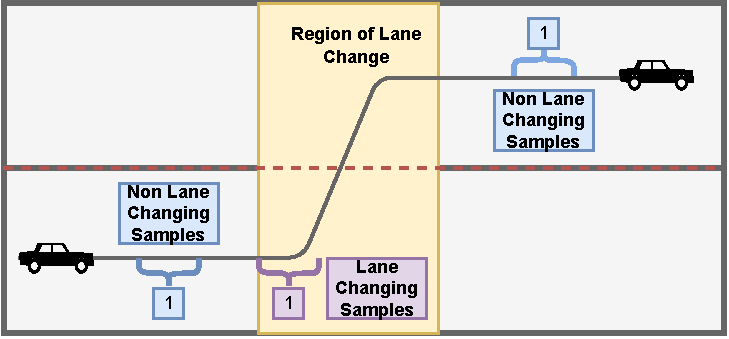
\includegraphics[width=\textwidth]{sections/motivation/fig/Sample_Extraction.pdf}
    \caption{Sample extraction from the NGSIM dataset.}
    \label{fig:extract}
\end{figure}

\begin{figure}
    \centering
    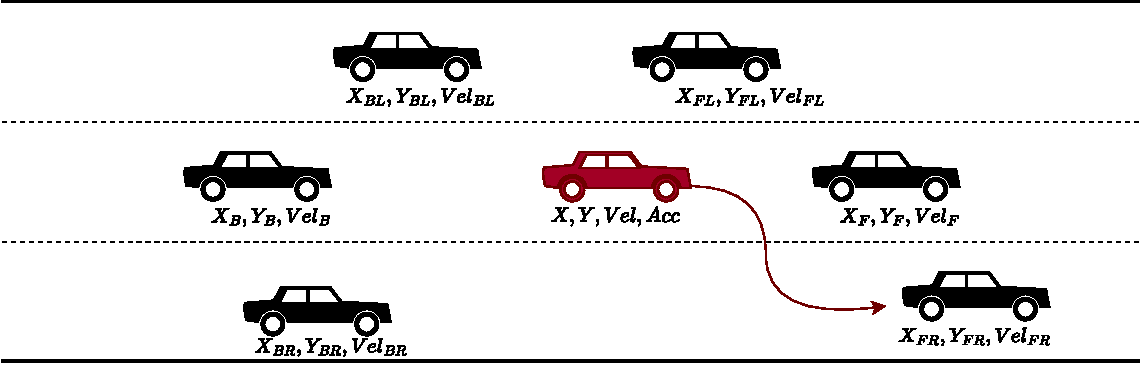
\includegraphics[width=\textwidth]{sections/compositional/fig/Car_Placement.pdf}
    \caption{Arrangement of cars and their important parameters before the red car can change lanes. The subscripts F, B, L and R refer to cars in the front, the back, the left and the right of the red subject vehicle, respectively. Variables $X$, $Y$, $Vel$, and $Acc$ refer to the position, velocity, and acceleration of the cars.}
    \label{fig:car_placement}
\end{figure}

The extracted dataset contains 16,676 sample points from 559 lane changing (LC) cars, each sample containing 22 parameters or features. There are 11,006 No LC (lane keep) samples (labelled 1), 4,380 Left LC samples (labelled 0) and 1,290 Right LC samples (labelled 2). The features that act as inputs to the models include the position of the ego car (2 features), its velocity (1 feature), its acceleration (1 feature), and the relative positions (12 features) and velocities (6 features) of surrounding vehicles as input parameters to the model. Finally, we label the dataset according to the number of classes.



\section{2-Stage Compositional Design for Classification}
\label{sec:Class}
Our method relies on the divisibility of a monolithic classification model on the classes that the model predicts. We decompose or divide a monolithic design with $C$ output classes into $C-1$ compositional models, where each model corresponds to a particular class. The motivation for this approach comes from the DLC case study, where the problem is to classify whether the current state of the subject vehicle is safe for a left, right or no lane change. When working on this problem's compositional idea, we discovered that we could work with ANN models for left and right lane changes and omit the one for no lane change. This omission is natural for humans, as we often arrive at a no lane change decision after failing to decide on left or right. Further, this is implementable because we can deduce the omitted class based on the outputs of the two models. 

The method we developed generalises this idea to classifications with more than three classes. The $C-1$ ANNs are developed such that a model corresponding to class $\text{C}$ will output a High (value $\geq$0.5) when the input to the model has the same class label; otherwise, the model will output a Low (value $<$0.5). Also, the models are constructed such that the sum of neurons in all $C-1$ models equals that of the monolithic design to ensure a fair comparison. This may mean that the individual compositional models may have a slightly different number of total neurons if the number of neurons in the monolithic case is not a multiple of the number of compositional models. However, the total number of neurons in a design will always remain the same in both designs. These ANNs run in parallel at the first stage, and their outputs are then passed onto a \emph{merge} model (in the second stage) that interprets these outputs and generates a single output value corresponding to any one of the $C$ class labels.

While it is also possible to add a model similar to the merge model at the end of the monolithic design to perform an \emph{argmax} operation (i.e. find the argument with the highest element) to produce a class with the highest probability, such an exercise is unnecessary. In contrast to the argmax operation, which is an integral part of the prediction step in a monolithic design, the merge model in the compositional design is added after the prediction step of individual compositional models. It performs the crucial task of producing a single output through conflict resolution among the outputs of the compositional models. Thus, while the monolithic design is just a single-stage design (with $C$ output nodes per model), the compositional design is a 2-stage pipeline (see Figure \ref{fig:comp_premise}). 

The outputs from the compositional models are passed onto a merge model that interprets these outputs and generates a single output value corresponding to any one of the $C$ class labels. We build the compositional models separately from the monolithic models and then combine the trained models using the merge model. 

This design method cannot be used for monolithic designs with fewer than three classes because, for two classes, both monolithic and compositional designs have a single model and hence become equivalent. While using $C$ models instead of the $C-1$ we use can eliminate this limitation, it can be expected to significantly affect the classification performance of the compositional design by reducing the number of neurons in the compositional models, since we try to maintain the same number of neurons between the monolithic and compositional designs. Also, an additional model can be expected to make the compositional design bulkier and harder to implement on hardware. 

This premise for developing compositional models is not specific to the case studies considered in this work. It applies to any feedforward ANNs used for classification problems with three or more classes. This includes a wide range of multidisciplinary classification problems, such as the classification of medical conditions, street signals, driving situations, and others, where this approach to compositional classification can be used.


\begin{figure}[htbp] 
 \centering
 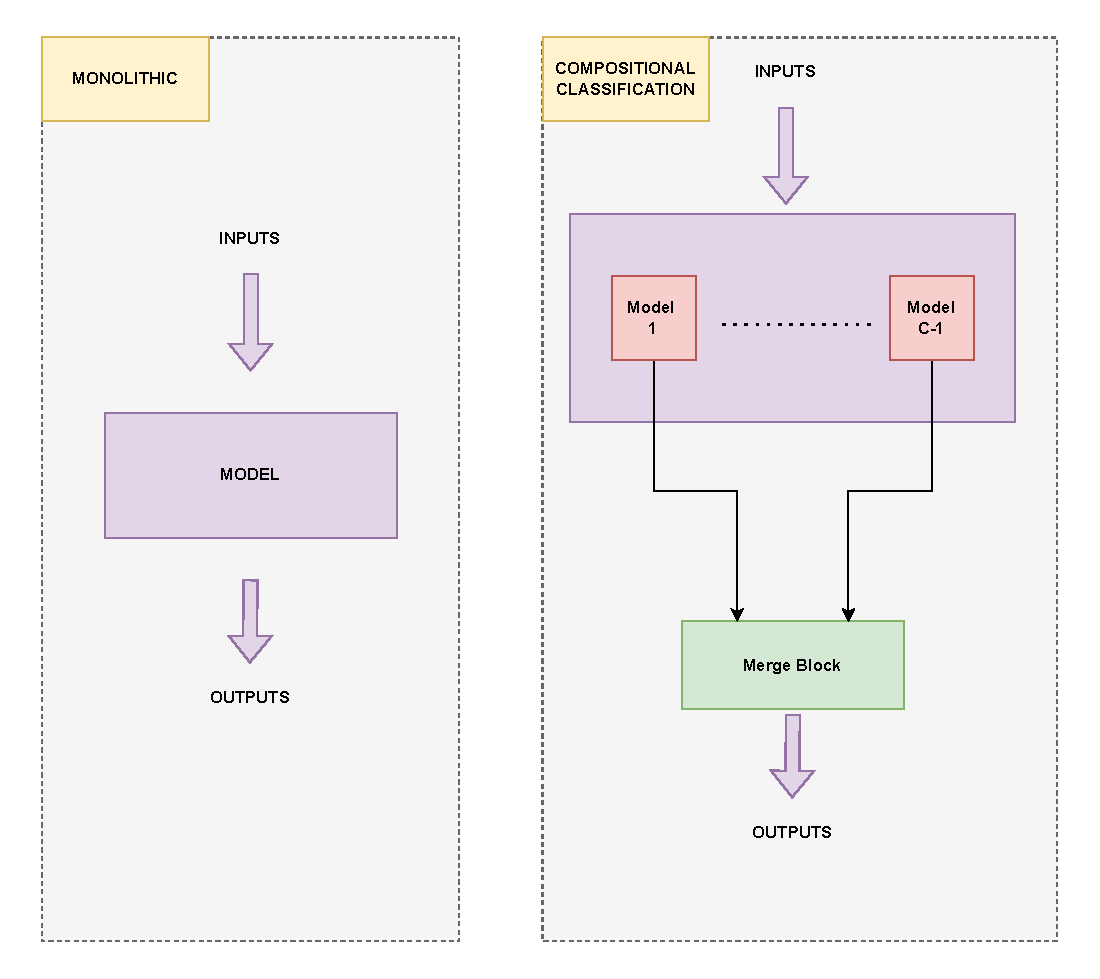
\includegraphics[width = \linewidth]{compositional/fig/comp_premise_class.pdf}
 \caption{Two-stage monolithic design and a 2-stage compositional design. We assume that we build models for the classes labelled $1,2,\cdots, C-1$, and the $C^{th}$ class is deduced as shown.}
 \label{fig:comp_premise}
\end{figure}



\subsection{Design Decisions}
\label{sec:sub_design_decisions}

The notion of compositionality for the classification models we use presents the following two main design-related questions. 

\begin{enumerate}
    \item Which $C-1$ classes should be chosen to build the compositional models?
    \item How do we divide the neurons among the compositional models to ensure equal total neurons in both designs and the lowest performance loss?
    \item How to combine the outputs of the compositional models, i.e., how to design the merge model?
\end{enumerate}

\begin{figure}
    \centering
    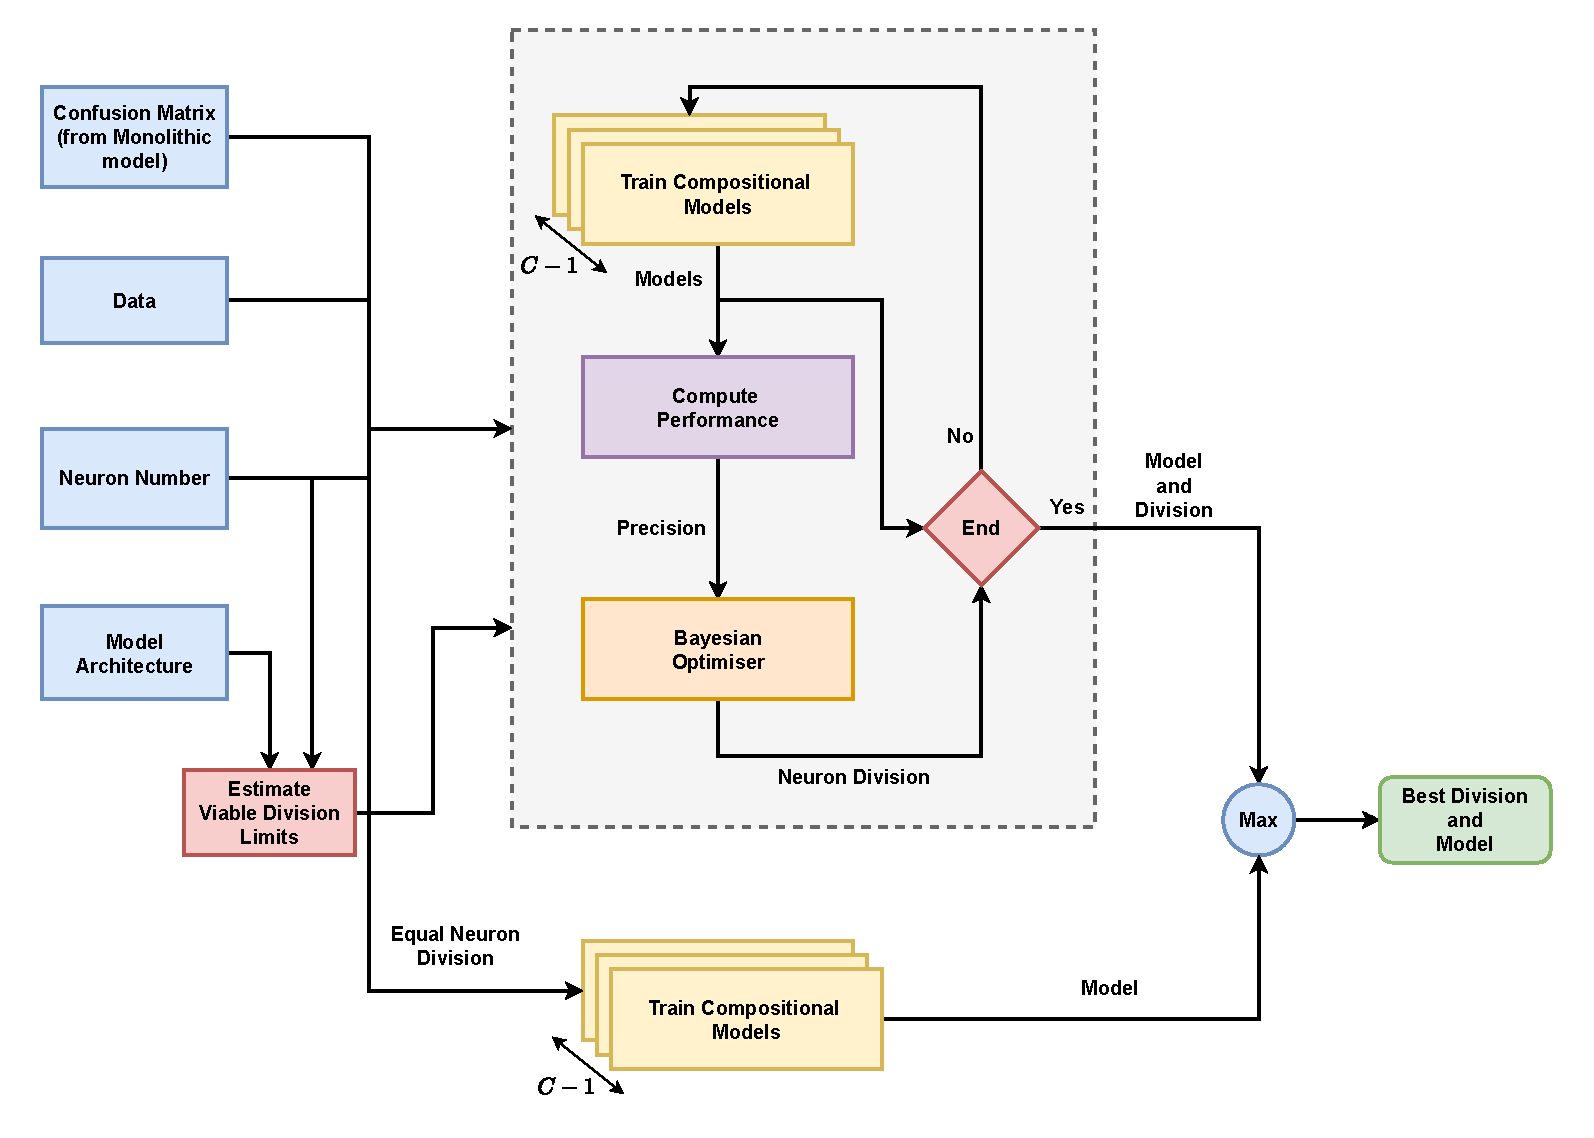
\includegraphics[width = \linewidth]{compositional/fig/Div_Optimisation.pdf}
    \caption{Diagram showing how using the $\text{confusion-matrix}$, the compositional models are chosen for training and optimised in a loop to maximise \textit{BalancedAccuracy} and find the best division of neurons between them. The neuron number (N) determines the total number of neurons in the design. The optimisation ends after 50 trials. Viable division limits are also computed to ensure model architecture constraints.}
    \label{fig:div_optimization}
\end{figure}

\subsubsection{Choosing Classes}
The division of the monolithic model into $C-1$ classes can be based either on domain (data) knowledge or on using qualitative and quantitative methods. For a more quantitative approach, we recommend using the $confusion-matrix$ we obtain from the monolithic design evaluation. Then, the diagonal of the matrix can be sorted to find the top $C-1$ easily classifiable classes and build models for them. A higher diagonal value implies higher ease in classifying the corresponding class. Building models for the $C-1$ easily classifiable classes should ensure that the remaining \textit{$C^{th}$} class is properly deduced by reducing the number of false positives from the trained models.


\begin{equation}
confusion-matrix = 
\begin{bmatrix}
TP_{1} & E_{1,2} & \cdots & E_{1, C}\\
E_{2,1} & TP_{2} & \cdots & E_{2, C}\\
\vdots & \vdots & \ddots & \vdots\\
E_{C, 1} & E_{C, 2} & \cdots & TP_{C}\\
\end{bmatrix}
\label{eq:conf_matrix}
\end{equation}

In Equation ~\ref{eq:conf_matrix}, $TP_{c}$ represents the number of true positives, i.e. the proportion of samples from class $c$ that were correctly classified as $c$, and $E_{c1, c2}$ represents the proportion of samples of class $c1$ that were incorrectly classified as $c2$. 


Similarly, the division of neurons among the $C-1$ models can be based on intuition/domain knowledge or a quantitative approach. We propose beginning with dividing the neurons equally between the chosen models and then deciding whether to optimise the neuron division among the models based on the performance of the compositional design vis-à-vis the monolithic design. A designer may choose a threshold for performance loss observed (if any) when migrating to a compositional design before opting for the optimisation route. This ensures that the compositional design is not over-engineered and that the performance loss is minimal.

We use the optimisation approach if the equally divided compositional design has a Precision loss of more than one per cent. We optimise the compositional design Precision using Bayesian optimisation with Gaussian processes \cite{mockus_bayesian_1975} while ensuring that the total number of neurons in the compositional models remains the same. 
% The procedure is shown in figure \ref{fig:div_optimization}. 
The optimisation can be stopped after a fixed number of trials or after the loss has attained a specific value. Also, any other suitable optimisation method, such as evolutionary algorithms, can be used in place of the one proposed, but the goal of optimising the model performance remains the same. 

In the general case, all the compositional models will share the same set of input features, i.e., those used by the monolithic design. However, if data domain knowledge can be used to remove a few redundant features in a few compositional models, it should be used to reduce the number of neurons in the compositional models, which can be beneficial for hardware implementation. 



\subsubsection{Dividing Neurons between models}

We either divide the neurons equally between the compositional models, or we optimise the top $C-1$ models such that the division of neurons between them maximises the Precision \cite{kelleher_fundamentals_2020} of the overall compositional system based on certain conditions.

For optimisation, we use Bayesian optimisation with Gaussian processes \cite{mockus_bayesian_1975} using the Latin Hypercube Sampling (LHS) \cite{mckay_comparison_1979} to generate random points for consideration. We use a function to provide architecturally viable limits for the division of neurons to the optimiser. This function is necessary to ensure that no model has any layers with zero neurons (which basically eliminates the layer). Although the optimisation procedure should eventually consider the case where we have an equal division of neurons (if this division corresponds to a nearby local or global minimum), the stochastic nature of the procedure makes it difficult to guarantee that this division will be considered in the finite number of optimisation steps/trials the procedure takes. Hence, we separately develop compositional models with equal division of neurons and take the compositional design with the maximum \textit{Precision} between the optimised and equally divided designs. The procedure is shown in Figure \ref{fig:div_optimization}. 

We can stop the optimisation after a fixed number of trials or after the performance (\textit{Precision}) has attained a specific value. In this work, we stop the optimisation after 50 trials. Also, any other suitable optimisation method, such as evolutionary algorithms, can be used instead of the one proposed, but the goal here remains the same. Moreover, we use optimisation only when the difference between the Precision of the monolithic design and the compositional design with equally divided neurons is more than 1\%. This is ensured by training the equally divided models first, which saves computational resources and time. 


\subsubsection{Designing the Merge Model}

The merge model can be designed to suit individual specifications. We illustrate the two ways used for two situations: (1) when choosing a model with decision conflict (more than one model predicting a High) is unsafe, and (2) when choosing a model with decision conflict is safe. For both ways, when only one of the $C-1$ compositional models produces a High, the merge module passes on the label for that model's class. Moreover, when none of them passes a High, i.e. none of the models is confident about its prediction, the label of the remaining $C^{th}$ class is passed as the output. 

\begin{equation}
  Out =\begin{cases}
  \text{C}_{safe} & \text{two or more Models output}  > 0.5\\
  1 & \text{if } \textsl{Model}_1 \text{ output} > 0.5 \text{ only}\\
  2 & \text{if } \textsl{Model}_2  \text{ output} > 0.5 \text{ only}\\
  \vdots & \\
  \text{C-1} & \text{if } \textsl{Model}_{C-1} \text{ output} > 0.5 \text{ only}\\
  \text{C} & \text{if all Model output} \leq 0.5
\end{cases}
\label{eq:merge1}
\end{equation}


However, when more than one model passes a High, the merge model in the safety-critical case (first case) outputs the label \text{C}$_{safe}$ of the class that can be used safely in a decision conflict (see Equation \ref{eq:merge1}). For the second case, where the output can be chosen between the conflicting models, the merge model outputs the label of the model with the maximum output value to allow the label of the most confident model to pass its output (see Equation \ref{eq:merge2}). This method enables the compositional classification of datasets with $C$ classes with just $C-1$ models. 


\begin{equation}
  Out =\begin{cases}
  \text{argmax(outputs)} & \text{two or more Models output}  > 0.5\\
  1 & \text{if } \textsl{Model}_1 \text{ output} > 0.5 \text{ only}\\
  2 & \text{if } \textsl{Model}_2  \text{ output} > 0.5 \text{ only}\\
  \vdots & \\
  \text{C-1} & \text{if } \textsl{Model}_{C-1} \text{ output} > 0.5 \text{ only}\\
  \text{C} & \text{if all Model output} \leq 0.5
\end{cases}
\label{eq:merge2}
\end{equation}

We can also use other mathematical functions, including ANNs, to combine the outputs of the compositional models. The ANN can be trained to learn the best combination of the outputs from the compositional models. It can be trained using the outputs from the compositional models as input and the actual output as the target using the backpropagation algorithm. However, we propose that we begin with the conditional merge model and then move to more complex merge blocks if the conditional merge model does not meet the performance requirements.


\subsection{Example}

Consider the 3-class classification problem from Figure \ref{fig:comp_premise_example} where we have a monolithic model that classifies the classes $0,1,2$. We can divide the monolithic model into two compositional models that classify the classes $0$ and $1$. Class $2$ is inferred based on the output of the two models. The merge model is designed as mentioned in \ref{eq:merge2}. The compositional model outputs the class label based on the output of the models. If both models output a value greater than $0.5$ (i.e., probability of more than $0.5$), the merge model outputs the class (either $C0$ or $C1$) label with the highest output value. If only one model outputs a value greater than $0.5$, the merge model outputs the class label of that model. If none of the models outputs a value greater than $0.5$, the merge model outputs the class label class $C2$. 

\begin{figure}[!htb]
    \centering
    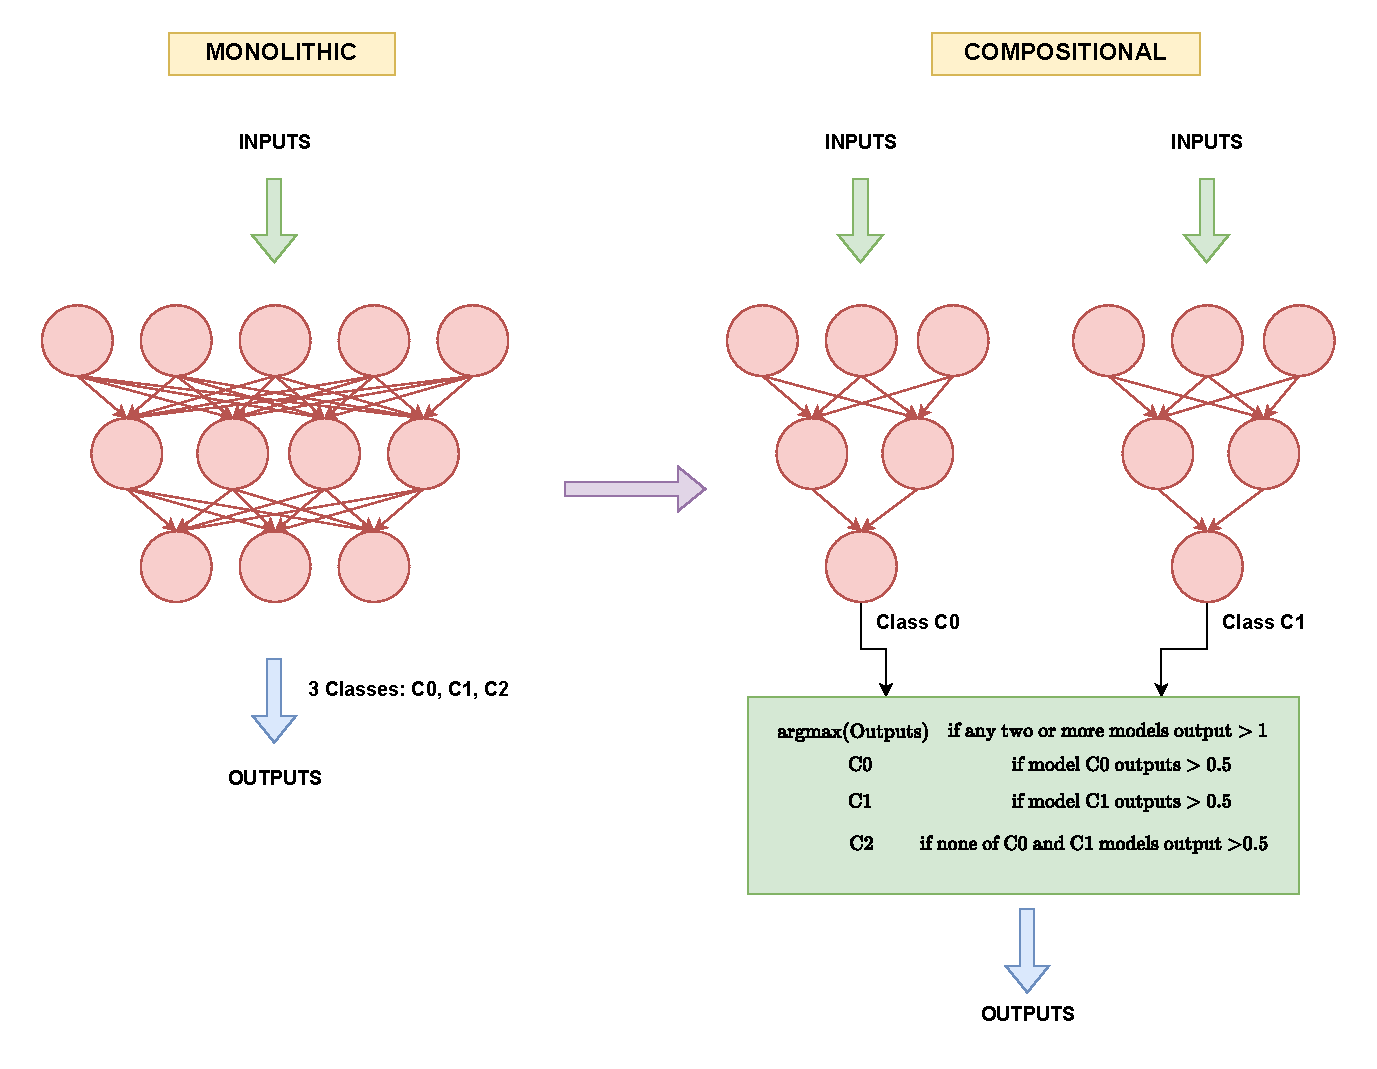
\includegraphics[width = \linewidth]{compositional/fig/Comp_Premise.pdf}
    \caption{Two-stage monolithic design and a 2-stage compositional design with three classes.}
    \label{fig:comp_premise_example}
\end{figure}

Compositional and monolithic models have the same number of neurons (12 neurons). Also, as can be seen from the figure, the monolithic model has three output nodes for the three output classes, while the compositional model has one output node each for the single class they learn to predict. Here, in this example, the input features are divided between the two models, but they can also be shared between the models.

\section{2-Stage Compositional Design for Regression}
\label{sec:Reg}

The compositional design for regression problems is similar to the classification problem, with a few differences. Since there are no classes in a regression problem, we do not divide the monolithic MLP design based on the values of the output feature. Here, we exploit the divisibility of the input feature set into individual compositional models. If the feature can be divided into $N$ clusters, we can build $N$ compositional models. 


\begin{figure}[htbp] 
    \centering
    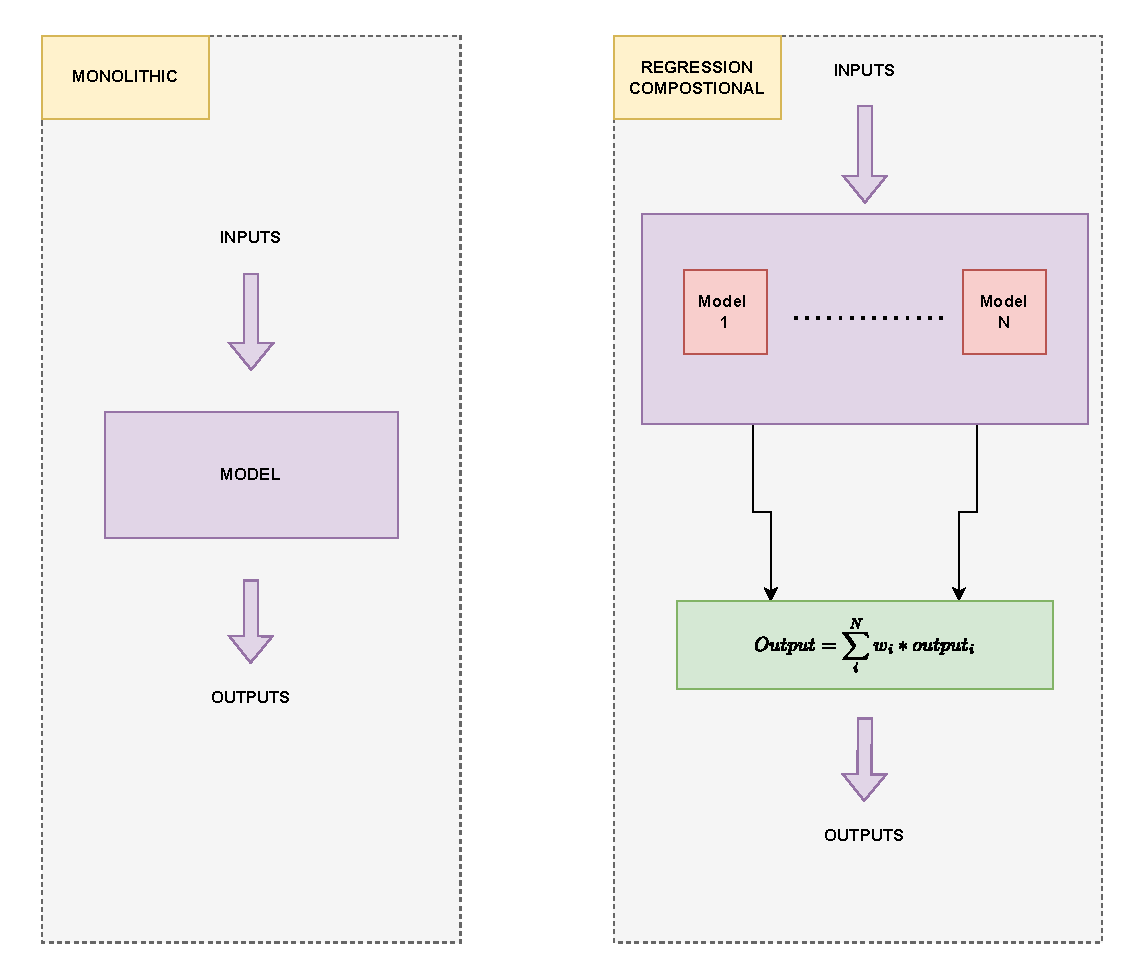
\includegraphics[width = \linewidth]{compositional/fig/comp_premise_reg.pdf}
    \caption{Single-stage monolithic design and a 2-stage compositional design. We assume that we build models for the clusters labelled $1,2,\cdots,N$.}
    \label{fig:comp_premise_reg}
   \end{figure}

Similar to the classification problem, the compositional design for the regression problem is also a two-stage design, with the first stage containing the $N$ compositional models (running in parallel) and the second merge stage combining the several model outputs into one (see Figure \ref{fig:comp_premise_reg}). The individual compositional models output a single continuous value. These are then combined using a mathematical function to output a single continuous value. 



\subsection{Design Decisions}

The notion of compositionality for regression models we use presents the following two main design-related questions.

\begin{enumerate}
    \item Which $N$ clusters should be chosen to build the compositional models?
    \item How do we divide the neurons among the compositional models to ensure equal total neurons in both monolithic and compositional designs, and the lowest performance loss?
    \item How do we combine the outputs of the compositional models?
\end{enumerate}

\subsubsection{Choosing the Feature Clusters}

We propose using data domain knowledge first to divide the input features into $N$ clusters. If domain knowledge is not available or does not achieve the same level of performance as the monolithic design, we recommend using a quantitative approach. We propose using the $K$-means clustering algorithm \cite{10.5555/1283383.1283494} to divide the input features into $N$ clusters. The $K$-means algorithm is a simple and efficient algorithm that can be used to partition the input features into $N$ clusters. The algorithm works by iteratively assigning each input feature to the nearest cluster and then recalculating the cluster centroids. The algorithm converges when the cluster assignments do not change or if the algorithm reaches a specified number of iterations.

Another way to cluster the input features is to use Hierarchical clustering with correlation as the distance metric. This method is useful when the number of clusters is not known beforehand. The algorithm works by iteratively merging the two closest clusters until only one cluster remains. The algorithm can be stopped at a specific number of clusters or when the distance between the clusters exceeds a certain threshold. 

Any other suitable clustering algorithm can also replace the clustering algorithms discussed. We can even use multiple algorithms to find the best set of features to keep in each cluster. We can begin by finding the best number of clusters, and then choose the best features to keep in each cluster by observing which features are most repeated in the clusters. Overall, the goal is to divide the input features into $N$ clusters that can be used to build the compositional models.


As we are dividing based on the features, the models in the compositional design will have a different number of features than the monolithic model, but the total number of features entering both designs will remain the same. The divided feature sets can be mutually exclusive or have repeated features. However, we advise using a set of mutually exclusive features to prevent feature redundancy, if that is desired, in the compositional models when we combine the models in the second step of the compositional design.


\subsubsection{Dividing the Neurons}

We either divide the neurons equally between the compositional models, or we optimise the top $N$ models such that the division of neurons between them minimises the \gls{mae}. We propose beginning with dividing the neurons equally between the chosen models and then deciding whether to optimise the neuron division among the models based on the performance of the compositional design vis-à-vis the monolithic design. A designer may choose a threshold for performance loss observed (if any) when migrating to a compositional design before opting for the optimisation route. This ensures that the compositional design is not over-engineered and that the performance loss is minimal.

We can use a similar methodology for performance optimisation as discussed in the classification section. We simply replace the performance metric Precision with \gls{mae} in the algorithm shown in Figure \ref{fig:div_optimization}. 



\subsubsection{Combining the Outputs}

We propose a weighted combination of the outputs from the compositional models (as a merge block) as shown in Equation \ref{eq:regression_combination} for a simpler hardware implementation. The weights of the weighted average are learned using backpropagation. We could also use a plain average of the outputs from the compositional models to further simplify the merge block.

\begin{equation}
output\_value = \sum_{i=1}^{n} w_{i} \times output_{i}
\label{eq:regression_combination}
\end{equation}

An ANN can also be used to replace the weighted combination of the outputs. The ANN can be trained to learn the best combination of the outputs from the compositional models. It can be trained using the outputs from the compositional models as input and the actual output as the target using the backpropagation algorithm. However, we propose that we begin with the weighted average merge block and then move to more complex merge blocks if the conditional merge block does not meet the performance requirements.

% \input{compositional/3stage.tex}





\section{Model Development}
\label{sec:sub_model}

We follow the following steps for MLP-based ANN design development of the datasets described. First, we pre-process the data with standard normalisation/scaling if it is not normalised, which modifies a dataset as shown in Equation \ref{eq:standard_scaler}. Second, we train the monolithic design model for different ANN architectures, as we do not have existing monolithic models for any of the example datasets considered. Third, we build the compositional design architecture.

When building the compositional design models, we can choose to have the same number of total neurons or different numbers in the two designs. While the former ensures a fairer performance comparison, we experiment with both approaches to comprehensively evaluate the two-stage compositional design. Finally, we train the compositional design with corresponding datasets using a 5-fold \gls{cv} method (from Section \ref{sec:intro_evaluation}). 

Moreover, we use the merge block in Equation \ref{eq:merge2} for the Small dataset models, as conflicts in these examples are not safety-critical. We use the merge block in Equation \ref{eq:merge1} for the DLC case study models, as choosing either the left LC or right LC model where conflict occurs can be unsafe. Here, we use the No Lane Change class as the \text{C}$_{safe}$ class (see Equation \ref{eq:merge1}). For the depression dataset regression models, we use the merge block in Equation \ref{eq:regression_combination}.

Additionally, we adopt random seed selection, best-model saving, and learning rate reduction practices to alleviate the undesirable effect of stochasticity (variability in model representations due to randomness) in training. The training of both the compositional and monolithic models is performed in Python using the well-known TensorFlow-Keras Library on a 64-bit Windows 10 system with Intel Core i7-9700CPU @ 3.00 GHz and 32 GB RAM. The following subsections discuss the specifics of developing models for the various datasets.



\subsection{Small Datasets}

We use a four-layer classification architecture for all monolithic and compositional designs for all three datasets. We ensure that the monolithic and compositional designs have the same total number of neurons. The Wine and Diabetes dataset monolithic designs have 24, 12, 6, and 3 neurons, while the Iris dataset monolithic model has 20, 10, 4 and 3 neurons in the four layers from input to output. Next, we find the classes to build the compositional models using the quantitative method mentioned in Section \ref{sec:sub_design_decisions}. 

We build compositional models for classes 0 and 1 for the Wine and Diabetes classes and classes 0 and 2 for the Iris dataset. We do not optimise the neuron division; instead, we divide the neurons equally between the two compositional models, as there was no performance loss. Further, we use \gls{tanh} for all layers except for the last layer, which uses Softmax for the monolithic model and Sigmoid for the compositional models. Also, both designs are trained for 200 epochs and a batch size of 8 for the Wine and Diabetes datasets and 4 for the Iris dataset.

\begin{table}
    \centering
    \caption{Parameter Values for the DLC Case Study}
    \begin{tabular}{cccccc}
    \hline
    Layers & Features (S) & \multicolumn{4}{c}{Total Neurons}\\
     & Mon./Com. &  \multicolumn{4}{c}{Varying N}\\
    \hline
    1 & 22/16 & 80 & 118 & 157 & 195\\
    3 & 22/16 & 80 & 118 & 157 & 195\\
    6 & 22/16 & 80 & 118 & 157 & 195\\
    10 & 22/16 & 80 & 115 & 157 & 192\\
    \hline
    \end{tabular}
    \label{tab:parameter_values}
\end{table}
  
    
\begin{table}[htbp]
    \centering
    \caption{Search values (or limits) for parameters during hyperparameter optimisation of the Depression Dataset. (N.A. means Not Applicable)}
    \label{tab:optimiser_values_comp}
    \begin{tabular}{|c|ccc|}
      \hline
      \multicolumn{4}{|c|}{\textbf{Monolithic}} \\
      \hline
      \textbf{Hyperparameter} & \textbf{Lower Limit} & \textbf{Upper Limit} & \textbf{Values} \\
      \hline
      Number of layers & 2 & 4 & N.A \\
      Neurons in input layer & 50 & 90 & N.A \\
      Activation & N.A & N.A & tanh, relu, elu, linear \\
      Batch size & N.A & N.A & 4, 6, 8 \\
      \hline
    \end{tabular}
  
    \begin{tabular}{|c|ccc|}
      \hline
      \multicolumn{4}{|c|}{\textbf{Compositional}} \\
      \hline
      \textbf{Hyperparameter} & \textbf{Lower Limit} & \textbf{Upper Limit} & \textbf{Values} \\
      \hline
      Number of layers & 2 & 4 & N.A \\
      Neurons in input layer & 10 & 15 & N.A \\
      Activation & N.A & N.A & tanh, relu, elu, linear \\
      Batch size & N.A & N.A & 4, 6, 8 \\
      \hline
    \end{tabular}
  \end{table}
  
    



\subsection{Depression Dataset Models}
We build personalised regression models for the Depression dataset, which contains data from seven human subjects. As it is usually challenging to build models on data collected from human biophysical signals due to their complexity, models often need to be optimised for their performance. Instead of manually choosing and tweaking a few parameters to obtain better performance, we choose Evolutionary Algorithm (EA) based algorithms to optimise the number of hidden layers in the model, the number of neurons in the input layer, the activation of the hidden layers, and the training batch size for both monolithic and compositional models. The designs are optimised for 50 iterations using \gls{mae} as the performance metric.

Once we have optimised the monolithic models, we divide the input feature into six mutually exclusive sets. We divide the features based on whether they refer to food, activity, sleep, physiological, psychological or neurocognitive feature sets and build compositional models for the sets. A compositional design contains these six models, which are trained and optimised separately and then combined using the merge block (from Equation \ref{eq:regression_combination}), the weights of which are learned using a gradient descent-based algorithm. The search parameters for the optimisation can be found in Table \ref{tab:optimiser_values_comp}. Regardless of the optimisation procedure, as we are making models for a regression problem, the final layer in the models for both designs always uses the $linear$ activation function.

Furthermore, we do not ensure that the compositional and monolithic designs have the same total neurons. However, we ensure that the neuron ranges for the compositional models are nearly a sixth of the monolithic model. This difference helps ascertain how well the compositional approach works when the total number of neurons in the compositional design differs from the monolithic design. 



\subsection{Discretionary Lane Change Case Study Models}

We built different monolithic and compositional classification designs for the DLC dataset, each with a different architecture. The Left and Right \gls{lc} classes are chosen for the compositional design based on observed DLC behaviour, and the No lane change class is left out. Moreover, we experiment with three values of total neurons, i.e. \{118, 157, 195\}, and different numbers of layers, i.e. \{1, 3, 6, 10\}, in the monolithic and compositional designs (see Table \ref{tab:parameter_values}).

Furthermore, we optimise the neuron division as the equal division of neurons between the models did not yield designs with good compositional performance. We optimise the designs using Bayesian optimisation based on the Precision of the compositional designs. We end the optimisation after 50 trials and use 20 initial points with LHS. We also experiment with a design with three models ($C$ models) and neurons equally divided among them for a more thorough comparison.

Moreover, while we have 22 features for the monolithic examples, we remove the features corresponding to cars on the right lane for the Left LC Model, and for the Right LC Model, we do the opposite. This feature reduction is justified as the vehicles travelling in the right lane have a limited impact on a driver's decision to change lanes to the left and vice versa. This reduction results in each compositional model having just 16 features. We should, however, note that the compositional design, on the whole, has the same number of inputs as the monolithic model. 

As each compositional model makes decisions for a single class, the model can have two labels. Each label corresponds to the probability of that model producing a High (corresponding to label 1) or Low (corresponding to label 0). For instance, we relabel the developed datasets when training a compositional model corresponding to class $\text{C}$. The samples corresponding to class $\text{C}$ are labelled 1, and the rest are labelled 0. This method contrasts with the labelling procedure described to train the monolithic model, where we have labels from $1$ to $C$ for a dataset with $C$ classes.





\section{Hardware Implementation}
\label{sec:hardware}


The implementation feasibility of the monolithic and compositional designs for all datasets on hardware is also essential when quantitatively evaluating their pros and cons. Therefore, we develop a compiler to compile the ANN designs (TensorFlow-Keras \cite{martin_abadi_tensorflow_2015} and PyTorch \cite{paszke_pytorch_2019-1} ANN designs) to \gls{vhdl} for implementation on a \gls{fpga} through a process adapted from \cite{allen_compositional_2019-1}. 

We develop the compiler (compiling TensorFlow-Keras ANN models to \gls{vhdl}) from scratch using techniques adapted from \cite{allen_compositional_2019-1}, particularly the pipelined multicyclic approach to ANN execution\footnote{The compiler can be imported in Python from https://test.pypi.org/simple/nn2vhdl==2.0.3}. This approach enables the reuse of neuron instances mapped into hardware to reduce the number of total hardware components needed for mapping and enables us to fit larger networks than would usually be possible. Furthermore, we extend the work in \cite{allen_compositional_2019-1} by adding support for compositional architectures and secondary ANN layers (like the Batch Normalisation layer) and more activation functions (such as \textit{softmax}, \textit{\gls{elu}}) which are implemented through discontinuous piecewise linear functions and \glspl{lut}. We also make the compiler generic enough to work with arbitrary model compositions, including the compositional paradigm discussed in this work. 

\begin{figure}[htbp]
    \centering
    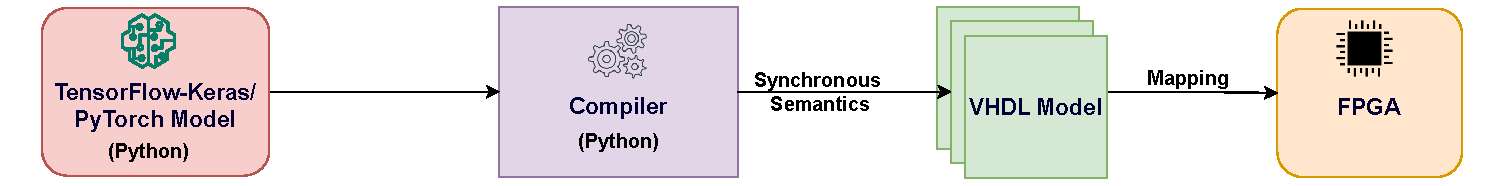
\includegraphics[width = \linewidth]{sections/compositional/fig/Compilation_Pipeline.pdf}
    \caption{Compilation pipeline for converting ANN designs to \gls{vhdl}.}
    \label{fig:comp_pipeline}
\end{figure}

The compilation pipeline can be seen in Figure \ref{fig:comp_pipeline}. In contrast to the work in \cite{allen_compositional_2019-1}, we develop the compiler in Python. This allows the compiler to be \textit{imported} (as a module) into existing Python-based ANN projects for easy compilation of ANN models. The compiler is widely applicable because Python is the most commonly used platform to develop ANN designs. It accepts both Tensorflow-Keras and Pytorch models or the weights and architectures of the models in an ANN design as its input. It compiles the design using synchronous semantics (explained in the next section) to a set of \gls{vhdl} files that execute the ANN design in a multicyclic manner. These files can be easily mapped onto any FPGA that accepts \gls{vhdl} designs. We call the hardware implementations of ANNs \glspl{hann}.

\subsection{Semantics of Hardware ANNs}
\label{sec:semantics}

\subsubsection{General Semantics}
To define the execution semantics of \gls{hann}, we borrow the structural semantic definitions used in \cite{allen_compositional_2019-1}. We begin by defining the concepts of delayed inputs and $\leftarrow$ or assignment. We denote the delayed semantics by the superscript $^P$ --- a process that introduces a slight delay but creates a deterministic operation. To further denote a cumulation of delays for $t$ time steps, the superscript notation $^{P^t}$ is used, with $t=1$ for a unit delay. We provide a mechanism for capturing the structural transformation from ANNs to these synchronous semantics used in HANN construction.

Firstly, at the lowest level, we provide the semantics for executing a single neuron. Each neuron takes some vector of inputs $\boldsymbol{I}$ and produces a single output $O$. Internally, the neuron has a set of weights $\boldsymbol{W}$ (where $|\boldsymbol{W}|=|\boldsymbol{I}|$) and a single bias $b$, and an arbitrary activation function $a$. The operation of a neuron with these properties is shown in Equation \ref{eq:kernel-neuron}, with the set of input values being from the previous tick, denoted by $\boldsymbol{I}^P$, as described earlier.

\begin{equation}
O \leftarrow a(\boldsymbol{W} \cdot \boldsymbol{I}^P + b)
\label{eq:kernel-neuron}
\end{equation}


The synchronous execution semantics of a HANN are such that data dependencies are broken at layer boundaries, meaning that individual neurons of a specific layer are executed each tick. The formal semantics of the operation of a HANN are presented using \gls{sos} rules \cite{plotkin_structural_2004-1} of the following form:
%
\begin{equation}
D \rightarrow D'
\label{eq:sos-form}
\end{equation}

where $D$ is the set of data variables before the transition, and $D'$ is the set of data variables after the transition.

Additionally, a further form of these semantics is used, which includes the option of including a predicate $p$ that must be satisfied for the rule to hold, as shown below.
%
\begin{equation}
\frac{p}{D \rightarrow D'}
\label{eq:sos-predicate-form}
\end{equation}

These transitions are composed together using synchronous semantics, allowing all neurons in a layer to be executed in lockstep with each other at the same rate, as determined by some global tick. Each neuron in the layer will execute a single computation transition per tick before synchronisation occurs, and the process repeats. During a tick, a neuron reads the inputs from the previous tick and executes them to generate the output. Also, delayed semantics provide a mechanism for dealing with data dependencies, as described before. This means that all variable reads of the system refer to values from the last tick (denoted by $^P$).

The semantics of a neural network is split into two parts: one which captures the mapping of values between neurons through weights and activation (Equation~\ref{eq:neuron-mapping}) and one which captures the parallel execution of transitions within a network (Equation~\ref{eq:parallel}). For Equation~\ref{eq:neuron-mapping}, which captures the mapping of values between neurons, $d_{i,l}$ is the output of the $i^{th}$ neuron in layer $l$ which is being assigned to, $d_{0,l-1}^P$ through $d_{n-1,l-1}^P$ are the output values from all $n$ neurons in the previous layer  $l-1$ and the previous tick. Finally, $f$ is a function that uses weights, biases, and activation to create the final sole output value. Indeed, Equation \ref{eq:neuron-mapping} represents the operation presented in Equation \ref{eq:kernel-neuron} in the SOS format.


\begin{equation}
    D \rightarrow D[d_{i,l} \leftarrow f(d_{0,l-1}^P, d_{1,l-1}^P, \dots, d_{n-1,l-1}^P)]
    \label{eq:neuron-mapping}
\end{equation}



Equation \ref{eq:parallel} captures the parallel execution semantics for each of the previously described transitions for neuron evolution and its mapping function. This parallel execution is used for all transitions within the same synchronous tick. Here, $d_{i,l}$ and $d_{j,l}$ represent two different data variables from two different neurons $i$ and $j$ at layer $l$ that are being modified through functions $f$ and $g$ respectively at the same instant. Here, all instances of $d$ in Equation \ref{eq:parallel} can either be an input or an output data variable, depending on the transition that is taking place. Due to the delayed semantics mentioned earlier, the two transitions can be combined into a single transition that performs two data-variable updates, regardless of their dependencies. For a multi-layer network, the semantics expressed by Equations \ref{eq:neuron-mapping} and \ref{eq:parallel} run across all layers until the final output is obtained.


\begin{equation}
    \frac{D \rightarrow D[d_{i,l} \leftarrow f(\dots)], D \rightarrow D[d_{j,l} \leftarrow g(\dots)], i \neq j}
    {D \rightarrow D[d_{i,l} \leftarrow f(\dots), d_{j,l} \leftarrow g(\dots)]}
    \label{eq:parallel}
\end{equation}



Additionally, it is essential to note that this rule is commutative and associative. Any arbitrary number of transitions can be executed at the same instant in time while all rules still hold.
Further, the commutation property means that these transitions may be specified in any order, and the overall system's output will be identical.


% \begin{theorem}
% \label{general_theorem}
% A single execution of a single feedforward HANN generated using the semantics described is deterministic, and it takes $L$ ticks to complete an execution, where $L$ is the number of layers in an HANN.
% \end{theorem}
% \noindent \textit{Informal Proof}: 
% We prove the theorem, a version of which exists in \cite{allen_compositional_2019-1}, using induction. We begin by considering an $L$-layer feedforward HANN $H$ with $i$ inputs, $L-1$ hidden layers with hidden neurons and $o$ output neurons in the output layer. 

% Per our delayed semantics, an input to $H$ at tick $0$ will be passed to the first hidden layer at tick $0$. However, this input will not be read until tick $1$ as the semantics demand that the input at the current layer is read from the previous tick to ensure that all inputs are present for computation. At tick $1$, the first hidden layer begins computation, generates its result, and passes its value to the next hidden layer, which will read this value at the next tick. This process repeats until the $(L-1)^{th}$ layer executes and produces an output at tick $L-1$. The output layer reads the result of the final hidden layer at tick $L$, and the output for the inputs at tick $0$ is finally produced. Thus, the process is completed deterministically layer-by-layer and takes $L$ ticks ($L$ layers).

% We can extend this operation for the case where the HANN execution begins at tick ${k}$ for any positive $k$ and guarantee determinism. This is because, irrespective of when the HANN execution begins, there are no cyclic data dependencies between the layers, i.e. the inputs to a layer at any tick are only dependent on the outputs from the previous tick or layer (if it exists) and not vice-versa. Similarly, for any starting tick value $k$, the layer-by-layer execution of the semantics ensures that a single execution process takes $L$ ticks to finish.

% Consequently, for any number of layers $L$ and any non-negative starting tick value $t$, $H$ is deterministic and completes its execution in exactly $L$ ticks. This result is further valid for HANNs with any number of inputs and outputs, as determinism is uninfluenced by these parameters.



\subsubsection{Compositional Semantics}
While these semantics can completely describe a monolithic design operation with a single HANN, the compositional design needs novel semantics for a multi-HANN two-level pipeline. For the first level, which consists of multiple HANNs, the process is similar to a single large HANN. Each HANN is executed in parallel with synchronisation at each tick using the associativity rule, which semantically results in each neuron in a tick being executed in parallel as shown in Equation \ref{eq:parallel}, where $f$ and $g$ can be neuron mapping functions from two different HANNs executing within the same layer.




\begin{equation}
    \frac{D \rightarrow D[d_{1} \leftarrow H_1(\cdots)], \dots, D \rightarrow D[d_{C-1} \leftarrow H_{C-1}(\cdots)]}
    { D \rightarrow D[O \leftarrow r(d_{1}^{P^{L-L_1+1}}, \cdots, d_{C-1}^{P^{L-L_{C-1}+1}})]}
    \label{eq:result-output}
\end{equation}



The semantics of the second level in the design can be obtained by combining the outputs from the compositional HANNs using a functional module that only executes when all preceding HANNs have finished executing. This requires delays, introduced using the superscript $^P$, to compensate for the different numbers of layers in the HANNs. We define the semantics as shown in Equation \ref{eq:result-output}, where $C$ is the number of classes; $H_{1}, \cdots, H_{C-1}$ represent the $C-1$ HANNs that map the network inputs to their respective outputs $d_{1}, \cdots, d_{C-1}$; $L_1, \cdots, L_{C-1}$ represent the number of layers in the HANNs; $L$ is the number of layers in the HANN that has the maximum number of layers; $^{P^{L-L_1 + 1}}, \cdots, ^{P^{L - L_{C-1}+1}}$ denote the delays we introduce to the outputs of individual HANNs to ensure deterministic operation with the additional $1$ ensuring that the merge block reads the outputs from the previous tick once all of them have been produced, and; $r$ represents the function that executes the merge block. $r$ maps the delayed outputs of HANNs to the single output variable $O$, and $O$ is the output of the entire compositional design. Thus, the semantics here ensure that all inputs to the merge function are delayed and read simultaneously, irrespective of the number of layers in the individual HANNs.


% \begin{theorem}
% \label{compositional_theorem}
% A single execution of a compositional HANN composed of $C-1$ feedforward HANNs generated using the semantics described is deterministic, and it takes $L+1$ ticks to complete an execution, where $L$ is the number of layers in the HANN that has the maximum number of layers.
% \end{theorem}
% \begin{proof}
% Consider a compositional HANN design $\textit{H}^C$ with $C-1$ individual feed-forward HANNs $H_1, \cdots, H_{C-1}$, each with $i$ inputs,  $L_1, \cdots, L_{C-1}$ hidden layers respectively, and $o$ output neurons in the output layer. 

% As per Theorem \ref{general_theorem}, all individual HANNs, $H_1, \cdots, H_{C-1}$, have deterministic executions and they each produce an output in $L_1, \cdots, L_{C-1}$ ticks respectively. Although the HANN with a lower $L$ will pass on its result sooner, the merge block's delayed semantics ensure that inputs are only read when all outputs from all HANNs are obtained. This means that all inputs to the merge block will be read-only after $L$ ticks (assuming all models start executing at tick 0), where $L$ is the number of layers in the HANN that has the maximum number of layers. Once all inputs are read at tick $L+1$, the merge block executes the values to determine a single output. Therefore, $H^C$ is deterministic for the case when $H^C$ starts at tick 0, and it takes $L+1$ ticks for $H^C$ to execute once.

% We can extend this operation for the case where the $H^C$ begins executing at tick ${k}$ for any positive $k$ as both the individual HANN executions and the merge operation are deterministic, with the latter not depending on the former. Therefore, for any number of HANNs with the maximum number of layers being $L$, and for any tick $k$, $H^C$ executes in a deterministic manner, and it completes its execution in exactly $k+L+1$ ticks.
% \end{proof}


\subsection{Multi-cycle Execution}
We use the semantics previously explained to explain the multi-cycle approach to HANN execution used in this work. In doing so, we extend the multi-cycle execution presented in \cite{allen_compositional_2019-1} with the compositional case. In multi-cycle execution, fewer neurons are instantiated in hardware, and multiple clock cycles are used for each execution tick. The set of internal variables for each neuron is stored in single-cycle memory, with each hardware instance of a neuron being fed one such set of variables each clock cycle. The neuron will read these variables, perform computation, and then write the updated output back to memory within one cycle. 

Subsequently, a counter will be incremented, which causes the neuron to read the next set of variables from memory in the next clock cycle. Once all required computations have been performed, the execution is complete, signifying the end of the tick. This will cause variables to be mapped to their subsequent neurons in the next layer and allow execution for the next tick to begin. Moreover, the number of cycles needed for a single execution is proportional to the maximum number of neurons of a particular type (activation).

This approach only changes how an HANN is operationally executed between ticks, from a single-cycle to a multi-cycle operation. This preserves the tick-based semantics of the execution presented in the sections before and, in turn, assures determinism in the HANN execution as before. Moreover, the reuse of neuron instances across multiple clock cycles in the multi-cycle approach results in an implementation with smaller logic requirements at the cost of increased computation time. Since modern FPGAs have reasonably high clock frequencies, the increase in computation time should be minimal. With this approach, we can synthesise larger networks in hardware while still allowing for the features that the semantics provide.





\subsection{Compilation of ANN design to VHDL}


The algorithms presented in Algorithms \ref{alg:nn2vhdl}, \ref{alg:parse}, \ref{alg:write-vhdl}, and \ref{alg:generate-vhdl} show the high-level pseudocode for the compiler. This compiler converts an Artificial Neural Network (ANN) design, which may consist of one or multiple ANN models, from popular deep learning frameworks (TensorFlow/Keras and PyTorch) into synthesisable \gls{vhdl} code using the multicyclic synchronous semantics described in the last two sections. To achieve this, an intermediate JSON representation is used to represent both the hierarchical inter-model (connections between models) and intra-model (connections within a model, i.e., between layers) dependencies and connections\footnote{The compiler only works for feedforward ANN designs using activations of type linear, \gls{tanh}, sigmoid, exponential, \gls{elu}, and \gls{relu} in MLP architectures}. 

The compiler operates through two key phases, as illustrated in Algorithm \ref{alg:nn2vhdl}:

\begin{enumerate}
    \item \textbf{Model Parsing} (Algorithm \ref{alg:parse}): Extracts architecture and weights from neural network models. This builds a JSON representation of the network topology.
    \item \textbf{\gls{vhdl} Code Generation} (Algorithms \ref{alg:write-vhdl} and \ref{alg:generate-vhdl}): Produces synthesizable \gls{vhdl} code with fixed-point arithmetic
\end{enumerate}


\begin{algorithm}[htbp]
    \caption{Compile TensorFlow/PyTorch Models to \gls{vhdl}}\label{alg:nn2vhdl}
    \begin{algorithmic}[1]
    \Function{nn2VHDL}{$models$, $conn$, $aParts$, $bSize$}
        %\Comment{Inputs:}
        %\Comment{$models$: List of models (architectures and weights).}
        %\Comment{$conn$: Connections between models.}
        %\Comment{$aParts$: Number of parts for piecewise activation functions.}
        %\Comment{$bSize$: Fixed-point bit size.}
        \State $jModel \gets$ \Call{parse}{$models$, $conn$, $aParts$, $bSize$}
        %\Comment{Parse models into a JSON representation.}
        \State $vhdlFiles \gets$ \Call{writeVHDL}{$jModel$}
        %\Comment{Generate \gls{vhdl} files from JSON representation.}
        \State \Return $vhdlFiles$
        %\Comment{Return generated \gls{vhdl} files.}
    \EndFunction
    \end{algorithmic}
\end{algorithm}




\subsubsection{Interface Algorithm}
The interface algorithm (Algorithm \ref{alg:nn2vhdl}) orchestrates the entire neural network to \gls{vhdl} conversion process. The algorithm consists of three main steps:

\begin{enumerate}
    \item \textbf{Line 2}: Calls the \texttt{parse} function to convert the input models into a structured JSON representation
    \item \textbf{Line 3}: Calls the \texttt{writeVHDL} function to generate \gls{vhdl} files from the JSON representation
    \item \textbf{Line 4}: Returns the complete set of generated \gls{vhdl} files
\end{enumerate}

The \texttt{nn2VHDL} function serves as the entry point for the compiler. It accepts the following inputs: 
\begin{itemize}
    \item \texttt{models} ($models$): A list of ANN models or the weights and architecture of the models in an ANN design.
    \item \texttt{conn} ($conn$): The interconnections between the models.
    \item \texttt{aParts} ($aParts$): The number of pieces/parts to use for approximating piecewise linear activation functions. 
    \item \texttt{bSize} ($bSize$): The bit size for the fixed-point representation used in computations. 
\end{itemize}


\begin{algorithm}[htbp]
    \caption{Parse Models to JSON Representation}\label{alg:parse}
    \begin{algorithmic}[1]
    \Function{parse}{$models$, $conn$, $aParts$, $bSize$}
        %\Comment{Convert models into a structured JSON representation.}
        \State $jModel \gets \{\}$
        \For{$model, model\_name$ \textbf{in} $models$}
            \State $mA \gets$ \Call{getModelArchitecture}{$model$}
            %\Comment{Extract model architecture.}
            \State $mW \gets$ \Call{getModelWeights}{$model$}
            %\Comment{Extract model weights.}
            \State $mAc \gets$ \Call{getPiecewiseAct}{$model$, $aParts$}
            %\Comment{Generate piecewise activation function definitions.}
            \State $mLc \gets$ \Call{getLayerConnection}{$model$}
            %\Comment{Extract layer connections.}
            \State $mJ \gets \{\text{``architecture"}: mA, \text{``weights"}: mW, \text{``act\_parts"}: mAc, \text{``layer\_conn"}: mLc\}$
            \State $jModel[model\_name] \gets mJ$
        \EndFor
        \State $jModel[\text{``conn"}] \gets conn$
        %\Comment{Store inter-model connections.}
        \State $jModel[\text{``fp\_size"}] \gets bSize$
        %\Comment{Store fixed-point bit size.}
        \State \Return $jModel$
    \EndFunction
    \end{algorithmic}
\end{algorithm}

\begin{algorithm}[htbp]
    \caption{Write \gls{vhdl} Files from JSON Representation}\label{alg:write-vhdl}
    \begin{algorithmic}[1]
    \Function{writeVHDL}{$jModel$}
        %\Comment{Generate \gls{vhdl} files from the JSON representation.}
        \State $modelVHDL \gets []$
        %\Comment{List to store model \gls{vhdl} files.}
        \State $aFile \gets []$
        %\Comment{List to store activation function \gls{vhdl} files.}
        \For {$conn$ \textbf{in} $jModel[\text{``conn"}]$}
            \For{$model\_names$ \textbf{in} {$conn$}}
                \State $mJ \gets jModel[model\_names]$
                %\Comment{Get JSON representation for the model.}
                \State $mVHDL \gets$ \Call{generateVHDL}{$mJ$}
                %\Comment{Generate \gls{vhdl} for the model.}
                \State $actVHDL \gets$ \Call{genActVHDL}{$mJ[\text{``act\_parts"}]$}
                %\Comment{Generate activation function \gls{vhdl}.}
                \State \textbf{append} $actVHDL$ \textbf{to} $aFile$
                \State \textbf{append} $mVHDL$ \textbf{to} $modelVHDL$
            \EndFor
        \EndFor
        \State $mFile \gets$ \Call{genModPipelineMap}{$modelVHDL$}
        %\Comment{Generate pipeline map for all models.}
        \State $lFile \gets$ \Call{genLibrary}{$jModel[\text{``fp\_size"}]$}
        %\Comment{Generate library for fixed-point arithmetic.}
        \State \Return $[mFile, aFile, lFile]$
        %\Comment{Return all generated files.}
    \EndFunction
    \end{algorithmic}
\end{algorithm}


\begin{algorithm}[htbp]
    \caption{Generate \gls{vhdl} Code Components}\label{alg:generate-vhdl}
    \begin{algorithmic}[1]
    \Function{generateVHDL}{$model$}
        \Comment{Convert a single model's JSON representation to \gls{vhdl} code.}
        \State \Return $vhdlCode$
    \EndFunction
    \Function{genActVHDL}{$activationParts$}
        \Comment{Generate \gls{vhdl} for piecewise linear activation functions.}
        \State \Return $activationVHDLCode$
    \EndFunction
    \Function{genModPipelineMap}{$modelVHDL$}
        \Comment{Generate a pipeline map for connecting models in \gls{vhdl}.}
        \State \Return $pipelineMapCode$
    \EndFunction
    \Function{genLibrary}{$fixedPointSize$}
        \Comment{Generate library files for fixed-point arithmetic.}
        \State \Return $libraryCode$
    \EndFunction
    \end{algorithmic}
\end{algorithm}


\subsubsection{Model Parsing Algorithm}
The model parsing algorithm (Algorithm \ref{alg:parse}) is responsible for extracting the neural network architecture from different deep learning frameworks. The algorithm operates as follows:

\begin{enumerate}
    \item \textbf{Line 3}: Initializes an empty JSON model structure
    \item \textbf{Lines 4-12}: Iterates through each model in the input list and extracts:
        \begin{itemize}
            \item \textbf{Line 5}: Model architecture via \texttt{getModelArchitecture}
            \item \textbf{Line 6}: Model weights via \texttt{getModelWeights}
            \item \textbf{Line 7}: Piecewise activation function definitions via \texttt{getPiecewiseAct}
            \item \textbf{Line 8}: Layer connections via \texttt{getLayerConnection}
        \end{itemize}
    \item \textbf{Line 9-10}: Constructs and stores a unified JSON representation for each model
    \item \textbf{Lines 13-15}: Adds global configuration including inter-model connections and fixed-point bit size
\end{enumerate}

The algorithm begins by detecting the framework type (PyTorch or TensorFlow/Keras) and routes to the appropriate parsing function. For PyTorch models, it traverses the computational graph to extract layer information, while for TensorFlow models, it analyses the model's layer structure directly. The algorithm then constructs a unified representation of the model architecture, including connections between layers and activation functions. It generates piecewise linear approximations for non-linear activation functions using Look-Up Tables (LUTs), which provide a resource-efficient mechanism for activation computation in hardware. For each activation function type, it calculates the appropriate derivative and constant terms needed for the linear approximation. The algorithm divides the function domain into a specified number of segments and computes the slope and intercept for each segment using the derivative at the midpoint.


\subsubsection{Compositional Model Parsing}
The compositional model parsing is handled within the main parsing algorithm (Algorithm \ref{alg:parse}). The algorithm handles complex neural network architectures composed of multiple interconnected models by:

\begin{enumerate}
    \item \textbf{Lines 4-12}: Processing each individual model independently to extract its architecture and components
    \item \textbf{Line 13}: Storing inter-model connections in the global JSON structure
    \item \textbf{Line 14}: Maintaining fixed-point configuration across all models
\end{enumerate}

This approach enables the conversion of sophisticated neural network systems that cannot be represented as a single sequential model by creating a unified representation that includes all individual models and their interconnections.

\subsubsection{VHDL Code Generation Algorithm}
The \gls{vhdl} code generation algorithm (Algorithm \ref{alg:write-vhdl}) transforms the JSON representation into synthesisable \gls{vhdl} code. The \gls{vhdl} mapping (from JSON) adopts a synchronous, multicyclic, and pipelined approach as discussed in Section \ref{sec:semantics}. This method reduces the hardware resources required for mapping by reusing neuron instances within the hardware. The algorithm operates as follows:

\begin{enumerate}
    \item \textbf{Lines 3-4}: Initialises lists to store model \gls{vhdl} files and activation function files
    \item \textbf{Lines 5-13}: Iterates through all connections and models:
        \begin{itemize}
            \item \textbf{Line 7}: Retrieves the JSON representation for each model
            \item \textbf{Line 8}: Generates \gls{vhdl} code for the model via \texttt{generateVHDL}
            \item \textbf{Line 9}: Generates activation function \gls{vhdl} via \texttt{genActVHDL}
            \item \textbf{Lines 10-11}: Appends generated files to existing model files
        \end{itemize}
    \item \textbf{Line 14}: Generates pipeline mapping for all models via \texttt{genModPipelineMap}
    \item \textbf{Line 15}: Generates fixed-point arithmetic library via \texttt{genLibrary}
    \item \textbf{Line 16}: Returns the complete set of \gls{vhdl} files
\end{enumerate}


The \gls{vhdl} code generation process is carried out by several key functions, as described in Algorithm \ref{alg:generate-vhdl}. The \texttt{generateVHDL} function converts a single model's JSON representation into \gls{vhdl} code, while \texttt{genActVHDL} produces \gls{vhdl} implementations for piecewise linear activation functions. The \texttt{genModPipelineMap} function is responsible for generating a pipeline map that connects the various models within the \gls{vhdl} design, and \texttt{genLibrary} creates the necessary library files to support fixed-point arithmetic operations.

Thus, the compilation system generates a complete \gls{vhdl} project structure that includes several key components: a main \gls{vhdl} file serving as the top-level entity with the full neural network implementation; a component library containing fixed-point arithmetic functions and utilities; individual \gls{vhdl} files for each activation function; and, optionally, a result processing block for classification tasks. Listing \ref{lst:usage_example} shows a basic usage example of the tool in Python.  
 

\begin{lstlisting}[language=Python, caption=Basic Usage Example of the compiler in Python, label=lst:usage_example]
# Import necessary libraries
from nn2vhdl import ToVHDL
from tensorflow.keras.models import Model
from tensorflow.keras.layers import Input, Dense

# Create a simple neural network
def create_model():
    inp = Input(shape = (16,), name = 'Input')
    x = Dense(int(16), activation = 'relu')(inp)
    x = Dense(int(8), activation  = 'relu')(x)
    x = Dense(int(4), activation  = 'relu')(x)
    out = Dense(1, activation = 'sigmoid')(x)

    model = Model(inp, out)
    # Compile model
    model.compile(optimizer = "adam", loss = 'binary_crossentropy')
    return model

# Create two models
modelL = create_model()
modelR = create_model()

# Convert Compositional ANN model to VHDL
ToVHDL(models=[modelL, modelR],
    \textsl{Model}_names = ["\textsl{Model}_L", "\textsl{Model}_R"], 
    connections = ["input[0:16] -> \textsl{Model}_L", "input[6:22] -> \textsl{Model}_R"], #Specify the connections between the models
    classes = [0,1,2], #Specify the labels of the classes
    max_inputs=22, #Specify the number of inputs
    result_block=True) #Specify if a merge block is required
\end{lstlisting}






\section{Results}
\label{sec:sub_results}



This section presents the results of the monolithic and compositional designs. We quantify the benefits and limitations of a compositional design against a monolithic design by comparing the predictive performance using F1-score for classification models and \gls{mae} for regression models, the hardware usage in terms of \glspl{alm} and the Worst-Case Execution Time (WCET) for the hardware implementations, and the number of computations and connections in the design. 

F1-score is the harmonic mean of the Recall and Precision, and produces a real number between 0 and 1. The \gls{mae}, as expected, is a real number over the entire real number domain. The performance of a classification (or regression) design is better if a design has a higher (or lower) F1-score (or \gls{mae}) value. Equations \ref{eq:F1}, \ref{eq:precision}, and \ref{eq:recall} define the F1-score, Precision, and Recall metrics, respectively. Since we use a 5-fold CV approach, we average the performance metrics across the five folds before the F1-score and \gls{mae} calculation.
    
Also, we found that using a 32-part piecewise linear approximation of the activation function and a 32-bit fixed-point representation of all numbers in the design, with 16 bits reserved for the fraction part, results in minimal performance loss due to loss in Precision when compiling the designs to VHDL. Furthermore, the \glspl{alm} are computed by fitting the developed VHDL designs onto the hardware of the Stratix-V FPGA using Quartus Prime Standard Version 19.1. We discontinue design fitting and call the design unsynthesisable if Quartus takes longer than 24 hours or if the design logic requirements are higher than the device can provide. In such instances, we report the ALM estimate as produced by Quartus but do not report the WCET, as it cannot be calculated. 

Additionally, the WCET is calculated from the maximum cycle frequency of the slow hardware synthesis model of Quartus for each design as shown in Equation \ref{eq:wcet}, where $f_{max}$ is the maximum cycle frequency of the design, and $N_{cycles}$ is the number of cycles required for a single execution of the design.


\begin{equation}
 WCET = \frac{N_{cycles}}
 {f_{max}}
    \label{eq:wcet}
\end{equation}

 

Finally, we compare the number of ANN computations, i.e. the number of additions and multiplications, and the number of connections encountered during one pass of a set of inputs. We report the percentage reduction in calculations and connections for the compositional design against the monolithic design.


\subsection{Best Neuron Divisions}

\begin{table}[hbt]
    \centering
    \caption{Best Neuron Divisions (DLC Dataset).
    (TN refers to the total number of neurons in the model. Left and Right refer to the compositional models for the Left and Right lane change classes. The values are the fraction of neurons in each model after optimisation.)}
    %\resizebox{\columnwidth}{!}{
    \begin{tabular}{|c|ccc|ccc|}
    \hline
    & \multicolumn{3}{c|}{1 Layer} & \multicolumn{3}{c|}{3 Layers} \\
    Models $\downarrow$ / TN $\rightarrow$ & 118 & 157 & 195 & 118 & 157 & 195 \\
    \hline
    Left & 0.69 & 0.71 & 0.74 & 0.62 & 0.54 & 0.51 \\
    Right & 0.31 & 0.29 & 0.26 & 0.38 & 0.46 & 0.49 \\
    \hline
    \end{tabular}%}% 
   
    %\resizebox{\columnwidth}{!}{ 
    \begin{tabular}{|c|ccc|ccc|}
    \hline
    & \multicolumn{3}{c|}{6 Layers} & \multicolumn{3}{c|}{10 Layers}\\
    Models $\downarrow$ / TN $\rightarrow$ & 118 & 157 & 195 & 115 & 157 & 192 \\
    \hline
    Left & 0.58 & 0.60 & 0.64 & 0.70 & 0.58 & 0.58 \\
    Right & 0.42 & 0.40 & 0.36 & 0.30 & 0.42 & 0.42 \\
    \hline
    \end{tabular}%}
    \label{tab:optimal_division}
\end{table}

Table \ref{tab:optimal_division} presents the results of the neuron division optimisation for the compositional models in the DLC dataset. In compositional design, the overall model is split into two sub-models, each responsible for predicting a specific class: the Left and Right lane change classes. The table shows, for a range of total neuron counts (TN) and different network depths (1, 3, 6, and 10 layers), the fraction of the total neurons allocated to each sub-model after the optimisation process. For example, with a single hidden layer and 118 total neurons, 69\% of the neurons are allocated to the Left model and 31\% to the Right model.  

Based on the values in Table~\ref{tab:optimal_division}, the optimal division of neurons between the Left and Right compositional models for the DLC dataset is not equal and varies depending on both the total number of neurons and the network depth. Across all configurations, the Left model consistently receives a higher fraction of neurons than the Right model, suggesting that the Left lane change class is more complex or requires greater model capacity to achieve optimal performance. Furthermore, we see a balanced division of neurons between the Left and Right models for higher layer counts and higher total neuron counts. This indicates that both the complexity of the classes and the architecture of the model influence the best allocation strategy.




\subsection{Computations and Connection Reduction}


\begin{figure}[htbp]
    \centering
    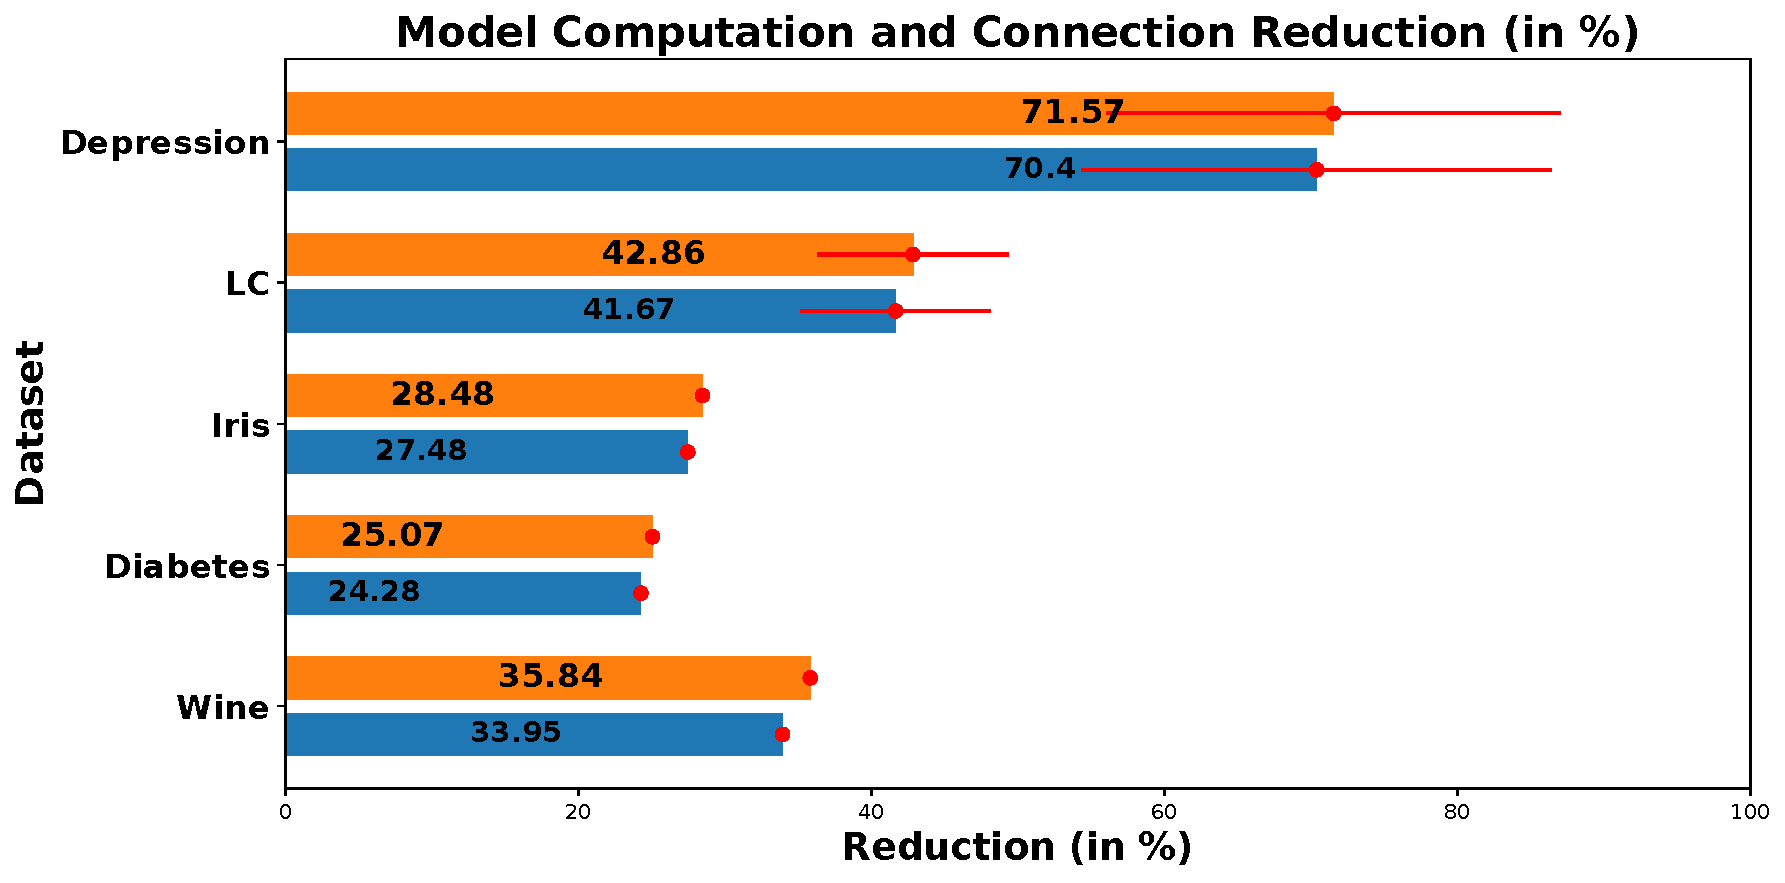
\includegraphics[width=\linewidth]{sections/motivation/fig/Model_Count_other_Red.pdf}
    \caption{ANN computation and connection reduction for the hardware ANNs for all datasets. The blue bars represent the percentage reduction in computations, whereas the orange bars represent the percentage reduction in connections when using a compositional design instead of a monolithic design. The Red bars show the variation in the values.}
    \label{fig:count_all}
\end{figure}


The percentage reduction in computations and connections for the compositional designs against the monolithic designs for all datasets is shown in Figure \ref{fig:count_all}. For brevity, we average the values across cases for both the DLC and Depression datasets. We observe that a compositional design results in an average reduction of computations and connections of 40\% over all datasets. This reduction is higher for bigger datasets and larger models, at around 40-70\%, and at least 24\% for smaller datasets. 

The Depression dataset has the highest reduction in computations and connections of around 70\% with a standard deviation of around 16\%, which can be attributed to a larger number of models per design and unequal neuron numbers between the monolithic and compositional designs. The DLC dataset has a reduction of around 40\% with a standard deviation of around 6\%. The Diabetes dataset has the lowest reduction in computations and connections, which can be attributed to its small design size.

Also, the reduction in connections and computations is similar across all datasets, as reducing the connections will also reduce the computations, and vice versa. This reduction in connections and computations corroborates the excellent hardware resource gains design we saw when using compositional in the previous subsections. 



\begin{figure}[htbp]
    \centering
    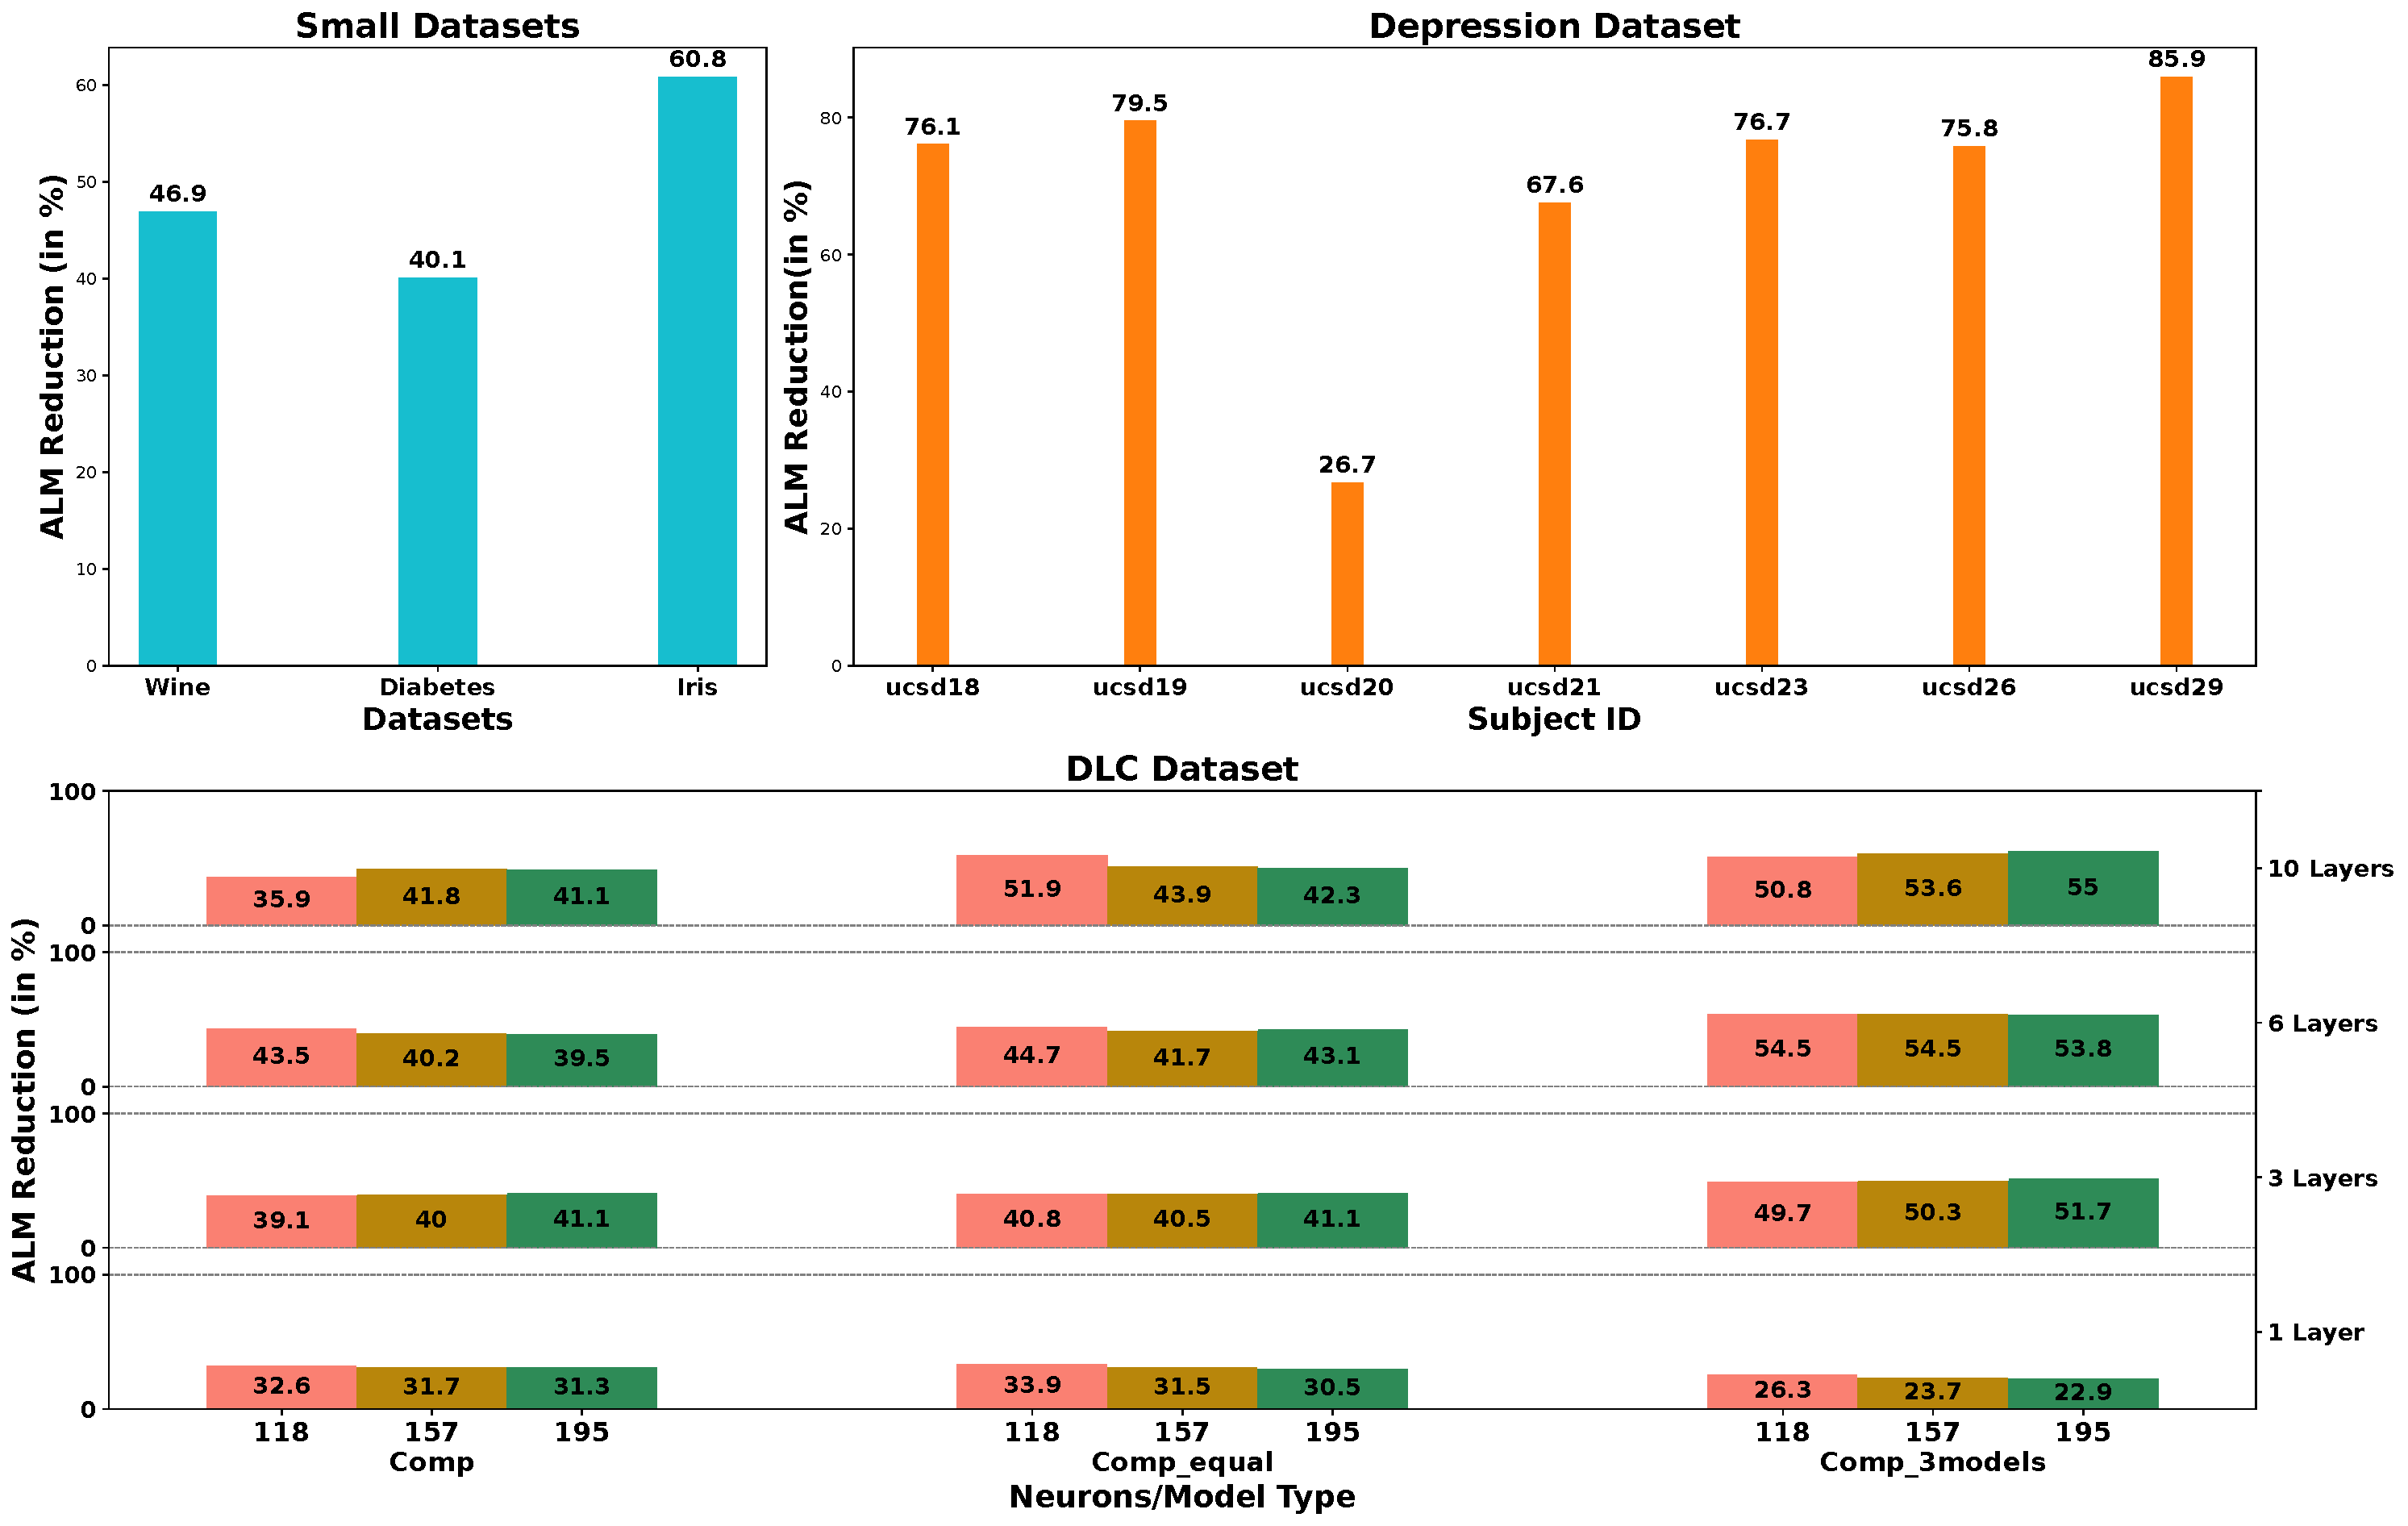
\includegraphics[width=\linewidth]{sections/motivation/fig/Model_ALM_Red.pdf}
    \caption{ALM reduction for all datasets. The blue bars represent the percentage reduction in ALM usage when using a compositional design instead of a monolithic design. The red bars show the variation in the values.}
    \label{fig:alm_all}
\end{figure}


\subsection{Hardware Performance}

Figure \ref{fig:alm_all} shows the ALM reductions for all datasets considered in this work. As we can see, the compositional design results in a hardware resource usage (measured using ALM usage) reduction of between 26 and 85 per cent, with an average reduction of 53.51 per cent across all datasets. Within the DLC dataset designs, the optimised compositional model and the equally divided compositional model seem to have similar ALM reductions and outperform the three-model compositional model. 

Furthermore, we see more variation in the ALM reduction in the Depression dataset, as the monolithic and compositional designs do not have the same number of total neurons. Especially for subject ucsd20, the decrease in ALM usage is only 26.7\%. This outlier is explained by the massive increase of 187\% in the total number of neurons used in the compositional design vis-à-vis the monolithic design, reducing the resource gain. Notably, despite this significant increase in the number of neurons between the designs, the compositional design still needs fewer hardware resources. 




\begin{figure}[htbp]
    \centering
    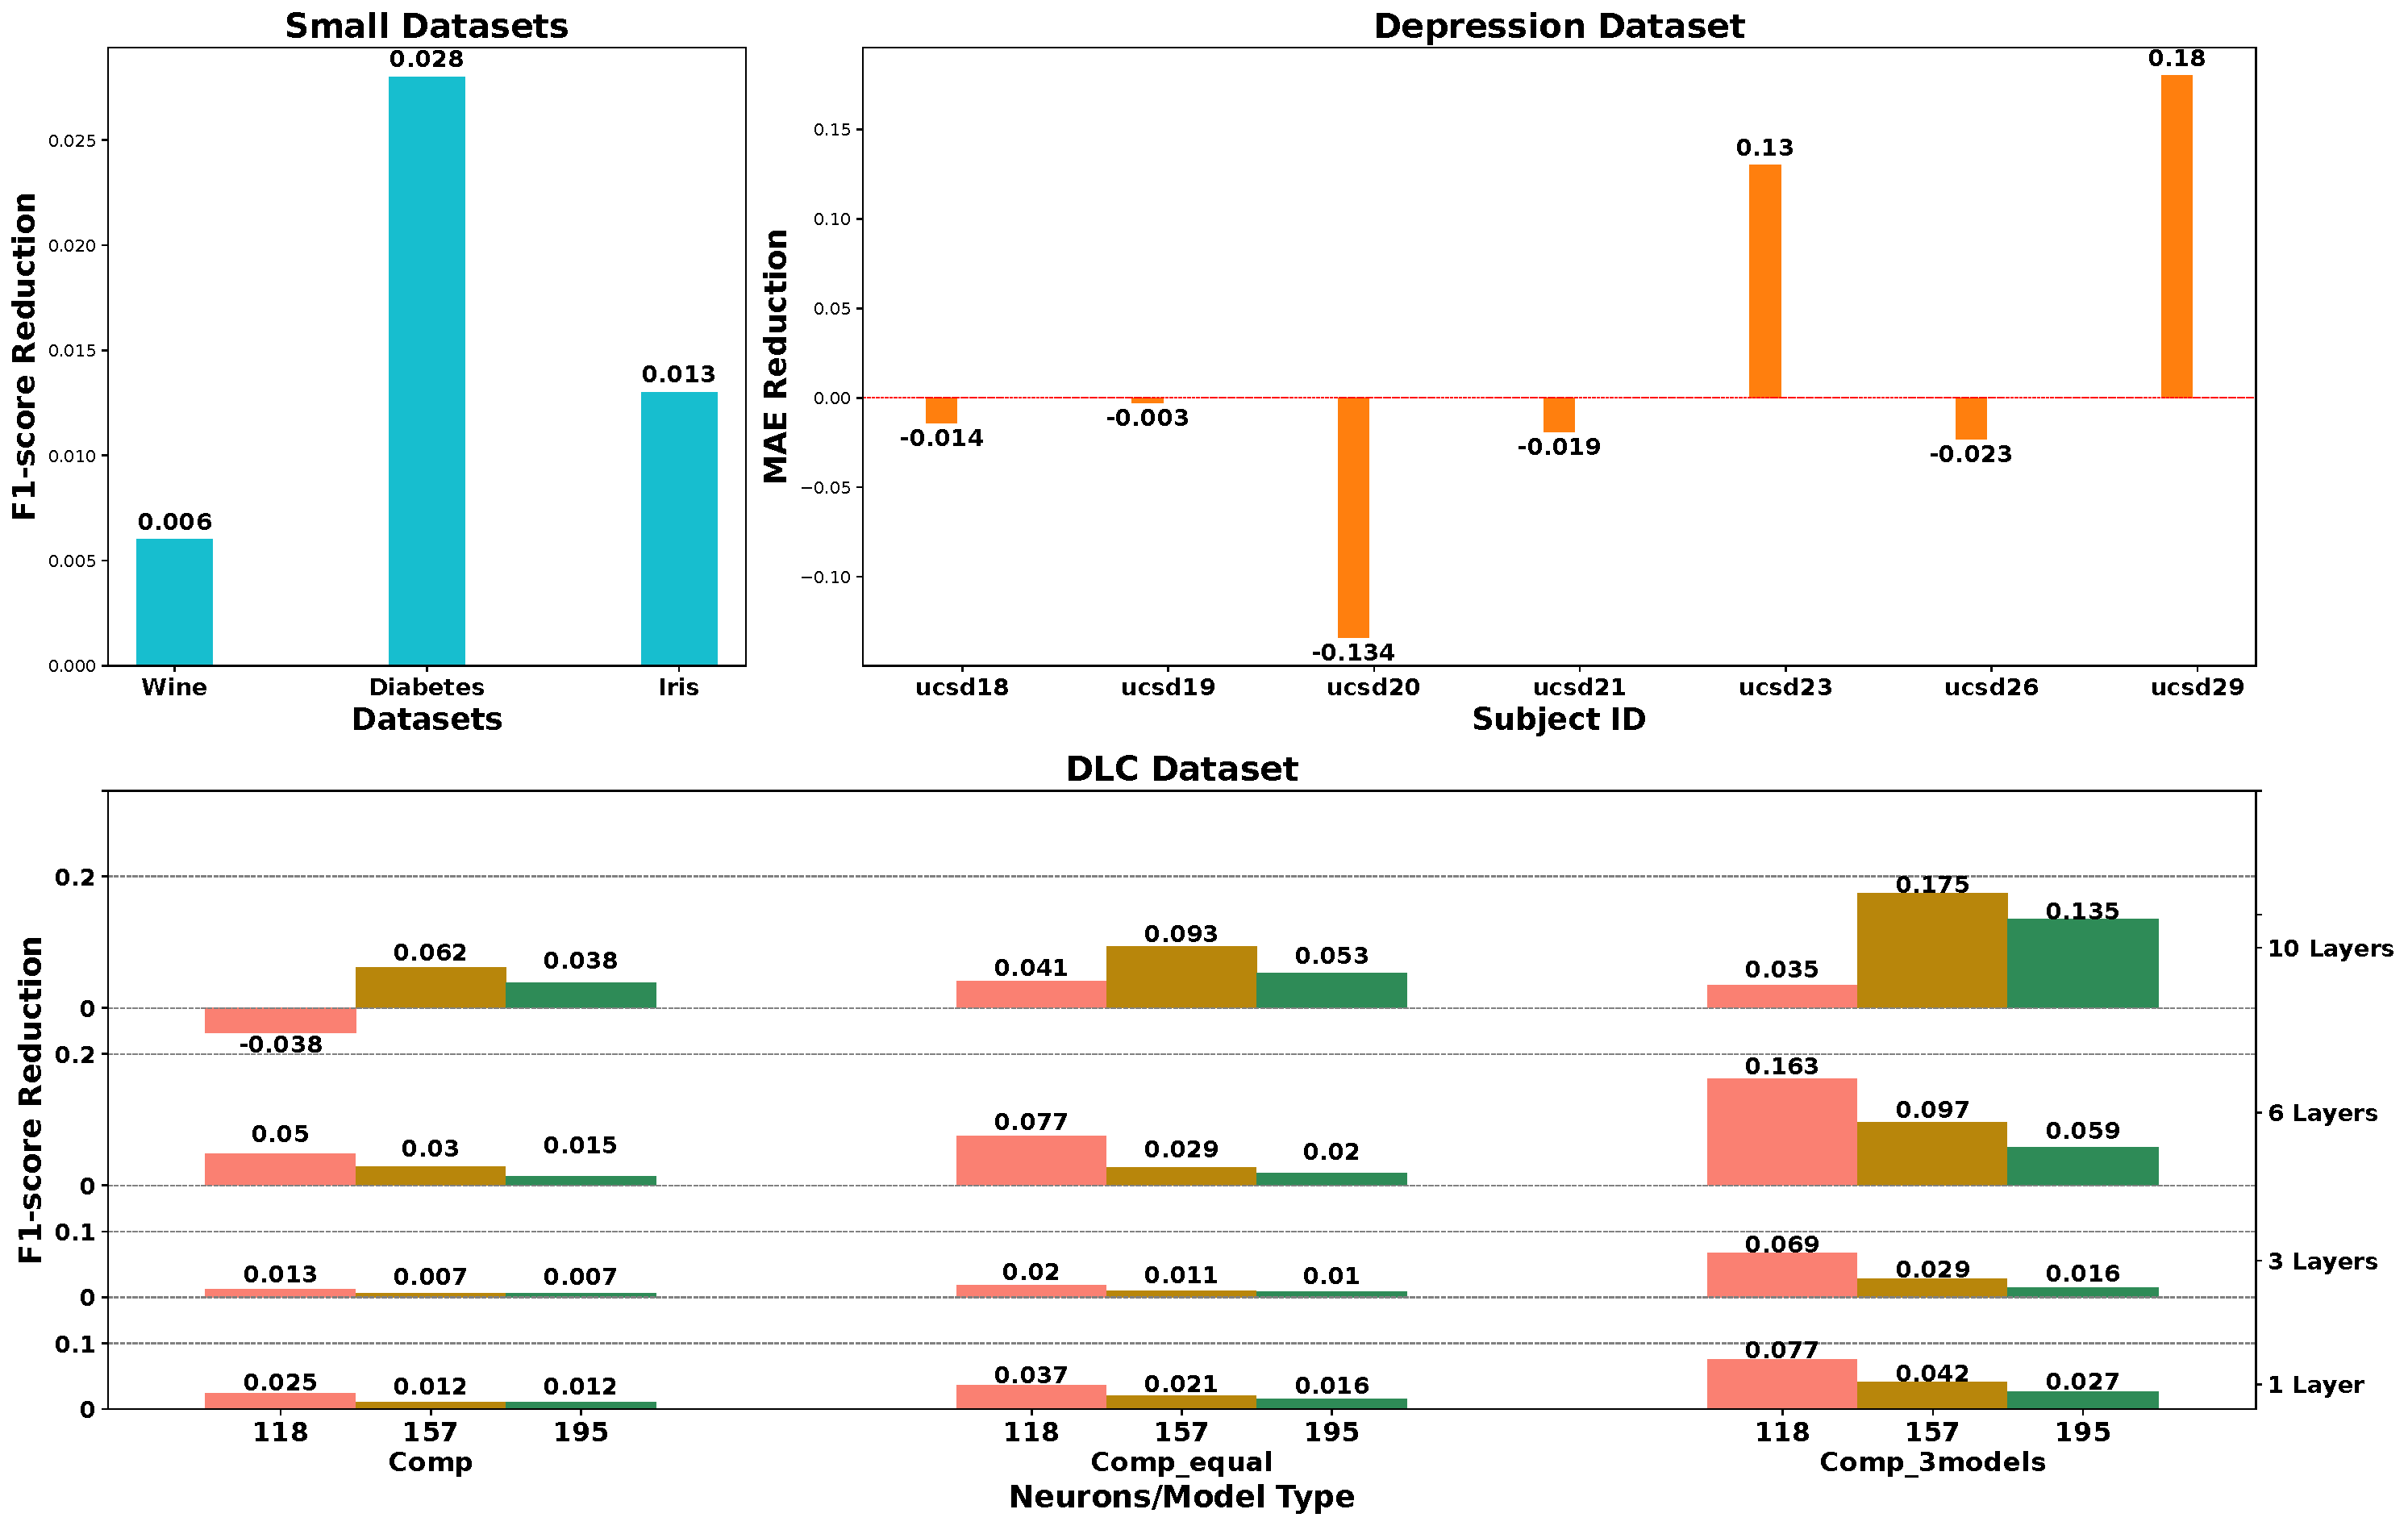
\includegraphics[width=\linewidth]{sections/motivation/fig/Model_Perf_Red.pdf}
    \caption{Predictive performance reduction (in absolute terms) for all datasets. Each bar plot refers to each small dataset in the Small Datasets plot. The bars in the Depression Dataset plot correspond to the seven human subjects (with anonymised names) considered. The DLC dataset plot is shown for various total neuron numbers, layer counts, and model combinations. "Comp" stands for the optimised compositional design, "Comp-equal" stands for the compositional design with an equal number of neurons between the compositional models, and "Comp-3models" stands for when the compositional design has three models with an equal number of neurons.}
    \label{fig:perf_all}
\end{figure}

\subsection{Predictive Performance}

Using a compositional design results in a minor reduction in designs' predictive performance for most designs and datasets, as shown in Figure \ref{fig:perf_all}. The reduction in F1-score for classification models is less than 0.1 for most designs, with the exception of the 3-model compositional design, where the reduction is around 0.2 for some cases. Within the DLC dataset designs, the optimised compositional model seems to perform the best. 

Also, as F1-score (which lies between 0 and 1) is generally less than 0.1, we can safely say that the reduction is less than 10\% for 92\% and is less than 5\% for 76\% of all classification designs. Moreover, the reduction in \gls{mae} for regression designs is less than 0.1 for 85\% of the subjects. As mood scores are integer values that range between 1 and 7, an absolute error/difference of 0.1 can be considered minor. Interestingly, designs for two subjects (ucsd23 and ucsd29) outperform the monolithic design. 


Further, the F1-score reduction shows a general decreasing trend for most designs for the DLC dataset, with the reduction decreasing as the number of neurons increases. As the number of neurons increases, the compositional design is able to learn the complex DLC dataset better and begins to catch up with the monolithic design in performance. One exception is the 10-layer design with 118 total neurons, where the compositional design marginally outperforms the F1-score of the monolithic design. Since this is an outlier, we attribute this performance to artefacts arising from randomness in the ANN architecture parameters.




\subsection{WCET Performance}


 
\begin{figure}[htbp]
    \centering
    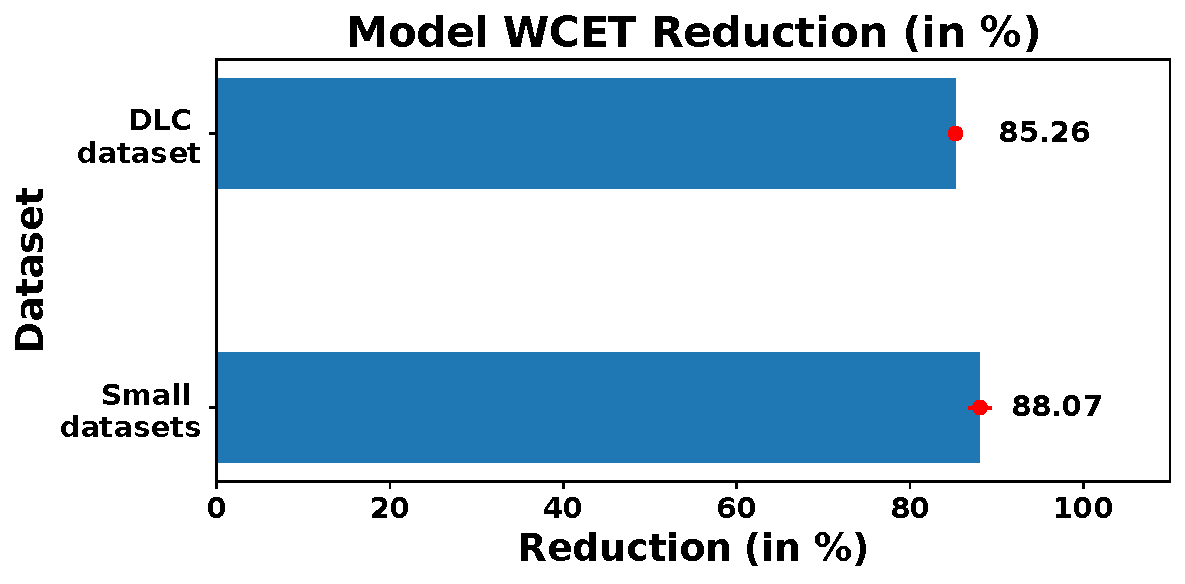
\includegraphics[width=\linewidth]{sections/motivation/fig/Model_WCET_red.pdf}
    \caption{Percentage WCET Reduction for the DLC dataset and the Small Datasets. The DLC and Small dataset reductions are averaged over their respective cases. The red error bars at the end show the variation in the values that have been averaged.}
    \label{fig:wcet_all}
\end{figure}


The percentage reduction in WCET for the compositional designs against the monolithic designs for the DLC and Small datasets is shown in Figure \ref{fig:wcet_all}. We averaged the percentage of WCET reduction across cases for both the DLC and small datasets, as they had minimal variation. We compute and average the WCET reduction for designs that are synthesisable. Overall, 47.22\% of the compositional and 25\% of the monolithic designs are synthesisable for the DLC dataset designs. All compositional and monolithic designs developed for the Small datasets were synthesisable. 

We can see from Figure \ref{fig:wcet_all} that the WCET reduction for both the DLC and Small datasets is around 85\%. This indicates a significant increase in the network speed for the compositional designs. As the compositional design has a much smaller fan-out of addition and multiplication components on hardware, compositional designs are significantly better in timing performance than monolithic designs. 

Furthermore, we found that none of the Depression dataset monolithic designs could be synthesised on hardware due to their high resource requirements. Hence, we could not compute the WCET reduction metric, and the results were not presented. Nevertheless, as all compositional models were synthesisable on hardware, we could compute the WCET of the compositional designs, which was around 1.4$\mu s$ for all subjects. 

\subsection{Summary of Results}

Overall, we make the following findings for the MLP-based ANN designs.

\begin{itemize}
    \item The compositional designs result in a significant reduction in hardware usage vis-à-vis monolithic designs with an average reduction of 53.51\% over all datasets at a minor reduction ($<$5\% for most designs) in performance. The reduction in performance decreases as the number of neurons increases.
    \item The compositional designs result in a massive reduction in WCET vis-à-vis monolithic designs with an average reduction of around 86\% over all datasets.
    \item The compositional designs significantly increase implementable designs vis-à-vis monolithic designs with an average increase of around 58\% over all datasets.
    \item The compositional designs significantly reduce design computations and neuron connections vis-à-vis monolithic designs with an average reduction of around 40\% over all datasets.
    \item The $C-1$ model compositional design performs better at ALM reduction and predictive performance reduction than the $C$ model compositional design for classification problems.
\end{itemize}


\subsection{Discussion}
We now discuss the intuition behind the observed results and comment on how far the conclusions extend beyond the datasets considered in this chapter.

The reductions in \glspl{alm}, WCET, and neuron connections shown in Figures \ref{fig:count_all}, \ref{fig:alm_all}, and \ref{fig:wcet_all} arise mainly from the structure of the compositional design rather than from properties unique to one application. A monolithic \gls{mlp} must implement all hidden neurons and connections on a single hardware datapath, which increases fan-out and critical-path length on the \gls{fpga}. In contrast, a compositional design runs several smaller ANNs in parallel (for classification) or on separate feature clusters (for regression) before applying a merge block. As we noted in Section \ref{sec:sub_results}, the compositional design has a much smaller fan-out of addition and multiplication components on hardware, which explains the large WCET reductions for the DLC and small datasets. Similarly, the average reduction of around 40\% in computations and connections is higher for bigger datasets and larger models, and lower when the monolithic baseline is already small, as in the Diabetes dataset.

We have also observed that using a compositional design results in only a minor reduction in predictive performance for most designs, as shown in Figure \ref{fig:perf_all}. This is expected because we maintain nearly the same total number of neurons between the monolithic and compositional designs while allowing each compositional model to specialise on a narrower sub-problem. For the DLC dataset, the neuron division in Table \ref{tab:optimal_division} allocates more neurons to the Left lane change model than to the Right model, which is consistent with the class imbalance described in Section \ref{sec:sub_datasets}. Furthermore, as the number of neurons increases, the compositional design learns the complex DLC dataset better, and the performance gap narrows. The Depression dataset shows the largest reductions in computations and connections, which can be attributed to the larger number of models per design and the fact that the number of neurons between the monolithic and compositional designs is not equal. 

We do not claim that every numerical result in this chapter will transfer unchanged to other datasets. Nevertheless, the qualitative trends---lower hardware usage, shorter WCET, fewer connections, and near-monolithic predictive performance---should hold for other feedforward \gls{ann} models in time-critical \glspl{cps} whenever the monolithic model is large enough to benefit from decomposition and the compositional split aligns with the structure of the problem (e.g., distinct classes or feature clusters). The DLC dataset is representative of a high-dimensional, imbalanced classification problem in transportation, whereas the small UCI datasets mainly illustrate the method at a modest scale. The Depression dataset highlights personalised regression models with limited data per subject, where compositionality improves implementability on hardware. The magnitude of the reported gains will depend on dataset size, class balance, model depth, and the decomposition strategy chosen.


\section{Summary}
\label{sec:chapter3_conclusions}
In this chapter, we present a novel application-agnostic approach to replacing single monolithic feedforward ANN designs with compositional designs composed of several smaller ANNs and use several examples and tests to examine the capabilities of each design, both on software and hardware. We illustrate the approach through a two-stage method to designing compositional ANNs and examine it against monolithic ANNs through multiple example datasets, including a depression dataset and a \gls{dlc} dataset. To aid in proper timing analysis using WCET, we develop a compiler that uses synchronous execution semantics to implement ANN designs on hardware. We further use a multicyclic approach that enables the reuse of hardware components and reduces the number of hardware resources required.

After a comprehensive comparison, we show that the very nature of compositionality makes it possible to significantly reduce the number of hardware resources (\glspl{alm}) required to synthesise the \gls{mlp}-based ANN models into hardware, specifically the Stratix-V FPGA board. Despite the minor performance loss, we discuss how a compositional design helps significantly reduce neuron connections, hardware resources and the WCET. The significant decrease in neuron connections and the overall size of individual models should also make verification easier. However, one of the key limitations of the approach is the need for an existing Monolithic model, which is a feedforward ANN and whose internal structure is known. Nevertheless, the method presented is not specific to the datasets presented and the type of \gls{ml} model considered in this chapter. We have only shown the 2-stage approach with \gls{mlp} models, where the merge block can be any relevant, arbitrary mathematical function; however, the compositional design allows for arbitrary combinations of different feedforward \glspl{ml} models as long as the input-output compatibility of the stages is maintained. We will explore more compositional design variants in the next two chapters. 







